% Options for packages loaded elsewhere
\PassOptionsToPackage{unicode}{hyperref}
\PassOptionsToPackage{hyphens}{url}
\PassOptionsToPackage{dvipsnames,svgnames,x11names}{xcolor}
%
\documentclass[
  letterpaper,
  12pt,
  oneside,
  spanish,
  doublespacing,
  headsepline,
  parskip]{MastersDoctoralThesis}

\usepackage{amsmath,amssymb}
\usepackage{lmodern}
\usepackage{iftex}
\ifPDFTeX
  \usepackage[T1]{fontenc}
  \usepackage[utf8]{inputenc}
  \usepackage{textcomp} % provide euro and other symbols
\else % if luatex or xetex
  \usepackage{unicode-math}
  \defaultfontfeatures{Scale=MatchLowercase}
  \defaultfontfeatures[\rmfamily]{Ligatures=TeX,Scale=1}
\fi
% Use upquote if available, for straight quotes in verbatim environments
\IfFileExists{upquote.sty}{\usepackage{upquote}}{}
\IfFileExists{microtype.sty}{% use microtype if available
  \usepackage[]{microtype}
  \UseMicrotypeSet[protrusion]{basicmath} % disable protrusion for tt fonts
}{}
\makeatletter
\@ifundefined{KOMAClassName}{% if non-KOMA class
  \IfFileExists{parskip.sty}{%
    \usepackage{parskip}
  }{% else
    \setlength{\parindent}{0pt}
    \setlength{\parskip}{6pt plus 2pt minus 1pt}}
}{% if KOMA class
  \KOMAoptions{parskip=half}}
\makeatother
\usepackage{xcolor}
\usepackage[paper=a4paper,inner=2.5cm,outer=2.5cm,bindingoffset=.5cm,top=2.5cm,bottom=2.5cm]{geometry}
\setlength{\emergencystretch}{3em} % prevent overfull lines
\setcounter{secnumdepth}{5}
% Make \paragraph and \subparagraph free-standing
\ifx\paragraph\undefined\else
  \let\oldparagraph\paragraph
  \renewcommand{\paragraph}[1]{\oldparagraph{#1}\mbox{}}
\fi
\ifx\subparagraph\undefined\else
  \let\oldsubparagraph\subparagraph
  \renewcommand{\subparagraph}[1]{\oldsubparagraph{#1}\mbox{}}
\fi


\providecommand{\tightlist}{%
  \setlength{\itemsep}{0pt}\setlength{\parskip}{0pt}}\usepackage{longtable,booktabs,array}
\usepackage{calc} % for calculating minipage widths
% Correct order of tables after \paragraph or \subparagraph
\usepackage{etoolbox}
\makeatletter
\patchcmd\longtable{\par}{\if@noskipsec\mbox{}\fi\par}{}{}
\makeatother
% Allow footnotes in longtable head/foot
\IfFileExists{footnotehyper.sty}{\usepackage{footnotehyper}}{\usepackage{footnote}}
\makesavenoteenv{longtable}
\usepackage{graphicx}
\makeatletter
\def\maxwidth{\ifdim\Gin@nat@width>\linewidth\linewidth\else\Gin@nat@width\fi}
\def\maxheight{\ifdim\Gin@nat@height>\textheight\textheight\else\Gin@nat@height\fi}
\makeatother
% Scale images if necessary, so that they will not overflow the page
% margins by default, and it is still possible to overwrite the defaults
% using explicit options in \includegraphics[width, height, ...]{}
\setkeys{Gin}{width=\maxwidth,height=\maxheight,keepaspectratio}
% Set default figure placement to htbp
\makeatletter
\def\fps@figure{htbp}
\makeatother
\newlength{\cslhangindent}
\setlength{\cslhangindent}{1.5em}
\newlength{\csllabelwidth}
\setlength{\csllabelwidth}{3em}
\newlength{\cslentryspacingunit} % times entry-spacing
\setlength{\cslentryspacingunit}{\parskip}
\newenvironment{CSLReferences}[2] % #1 hanging-ident, #2 entry spacing
 {% don't indent paragraphs
  \setlength{\parindent}{0pt}
  % turn on hanging indent if param 1 is 1
  \ifodd #1
  \let\oldpar\par
  \def\par{\hangindent=\cslhangindent\oldpar}
  \fi
  % set entry spacing
  \setlength{\parskip}{#2\cslentryspacingunit}
 }%
 {}
\usepackage{calc}
\newcommand{\CSLBlock}[1]{#1\hfill\break}
\newcommand{\CSLLeftMargin}[1]{\parbox[t]{\csllabelwidth}{#1}}
\newcommand{\CSLRightInline}[1]{\parbox[t]{\linewidth - \csllabelwidth}{#1}\break}
\newcommand{\CSLIndent}[1]{\hspace{\cslhangindent}#1}

\usepackage[utf8]{inputenc} % Required for inputting international characters
%\usepackage[T1]{fontenc} % Output font encoding for international characters; causes problems for xelatex

%\usepackage{mathpazo} % Use the Palatino font by default
\usepackage{fontspec}
\setmainfont{Arial}

\usepackage[backend=bibtex, style=authoryear, natbib=true]{biblatex} % Use the bibtex backend with the authoryear citation style (which resembles APA)

\usepackage[autostyle=true]{csquotes} % Required to generate language-dependent quotes in the bibliography



%----------------------------------------------------------------------------------------
%	MARGINS
%----------------------------------------------------------------------------------------

\geometry{
	headheight=4ex,
	includehead,
	includefoot
}

\raggedbottom

\AtBeginDocument{
\hypersetup{pdftitle=\ttitle} % Set the PDF's title to your title
\hypersetup{pdfauthor=\authorname} % Set the PDF's author to your name
\hypersetup{pdfkeywords=\keywordnames} % Set the PDF's keywords to your keywords
}
\usepackage{booktabs}
\usepackage{longtable}
\usepackage{array}
\usepackage{multirow}
\usepackage{wrapfig}
\usepackage{float}
\usepackage{colortbl}
\usepackage{pdflscape}
\usepackage{tabu}
\usepackage{threeparttable}
\usepackage{threeparttablex}
\usepackage[normalem]{ulem}
\usepackage{makecell}
\usepackage{xcolor}
\makeatletter
\makeatother
\makeatletter
\@ifpackageloaded{bookmark}{}{\usepackage{bookmark}}
\makeatother
\makeatletter
\@ifpackageloaded{caption}{}{\usepackage{caption}}
\AtBeginDocument{%
\ifdefined\contentsname
  \renewcommand*\contentsname{Tabla de contenidos}
\else
  \newcommand\contentsname{Tabla de contenidos}
\fi
\ifdefined\listfigurename
  \renewcommand*\listfigurename{Listado de Figuras}
\else
  \newcommand\listfigurename{Listado de Figuras}
\fi
\ifdefined\listtablename
  \renewcommand*\listtablename{Listado de Tablas}
\else
  \newcommand\listtablename{Listado de Tablas}
\fi
\ifdefined\figurename
  \renewcommand*\figurename{Figura}
\else
  \newcommand\figurename{Figura}
\fi
\ifdefined\tablename
  \renewcommand*\tablename{Tabla}
\else
  \newcommand\tablename{Tabla}
\fi
}
\@ifpackageloaded{float}{}{\usepackage{float}}
\floatstyle{ruled}
\@ifundefined{c@chapter}{\newfloat{codelisting}{h}{lop}}{\newfloat{codelisting}{h}{lop}[chapter]}
\floatname{codelisting}{Listado}
\newcommand*\listoflistings{\listof{codelisting}{Listado de Listados}}
\makeatother
\makeatletter
\@ifpackageloaded{caption}{}{\usepackage{caption}}
\@ifpackageloaded{subcaption}{}{\usepackage{subcaption}}
\makeatother
\makeatletter
\@ifpackageloaded{tcolorbox}{}{\usepackage[many]{tcolorbox}}
\makeatother
\makeatletter
\@ifundefined{shadecolor}{\definecolor{shadecolor}{rgb}{.97, .97, .97}}
\makeatother
\makeatletter
\makeatother
\ifLuaTeX
\usepackage[bidi=basic]{babel}
\else
\usepackage[bidi=default]{babel}
\fi
\babelprovide[main,import]{spanish}
% get rid of language-specific shorthands (see #6817):
\let\LanguageShortHands\languageshorthands
\def\languageshorthands#1{}
\ifLuaTeX
  \usepackage{selnolig}  % disable illegal ligatures
\fi
\IfFileExists{bookmark.sty}{\usepackage{bookmark}}{\usepackage{hyperref}}
\IfFileExists{xurl.sty}{\usepackage{xurl}}{} % add URL line breaks if available
\urlstyle{same} % disable monospaced font for URLs
\hypersetup{
  pdftitle={El efecto de la pandemia del COVID-19 en las condiciones de vida de las familias de trabajadores del sector informal en el Perú urbano},
  pdfauthor={Sotelo Galindo, Santiago Salvador},
  pdflang={es},
  colorlinks=true,
  linkcolor={black},
  filecolor={Maroon},
  citecolor={blue},
  urlcolor={blue},
  pdfcreator={LaTeX via pandoc}}

\thesistitle{El efecto de la pandemia del COVID-19 en las condiciones de
vida de las familias de trabajadores del sector informal en el Perú
urbano} % Your thesis title, this is used in the title and abstract, print it elsewhere with \ttitle
\supervisor{Sulmont Haak, David Jose
Antonio} % Your supervisor's name, this is used in the title page, print it elsewhere with \supname
\examiner{} % Your examiner's name, this is not currently used anywhere in the template, print it elsewhere with \examname
\degree{Licenciado en
Sociología} % Your degree name, this is used in the title page and abstract, print it elsewhere with \degreename
\author{Sotelo Galindo, Santiago
Salvador} % Your name, this is used in the title page and abstract, print it elsewhere with \authorname
\addresses{} % Your address, this is not currently used anywhere in the template, print it elsewhere with \addressname

\subject{} % Your subject area, this is not currently used anywhere in the template, print it elsewhere with \subjectname

\keywords{informalidad, pandemia, condiciones de
vida} % Your keywords, this is used in the title page and abstract, print it elsewhere with \keywordname

\city{Lima} % Your city's name, this is used in the title page and abstract, print it elsewhere with \cityname

\dateyear{2023} % Your year, this is used in the title page and abstract, print it elsewhere with \dateyearname

\university{}

\department{}

\group{}

\faculty{Facultad de Ciencias
Sociales} % Your faculty's name and URL, this is used in the title page and abstract, print it elsewhere with \facname

\setcounter{tocdepth}{1} % The depth to which the document sections are printed to the table of contents
\begin{document}
\pagestyle{empty} % Default to the plain heading style until the thesis style is called for the body content
\pagenumbering{gobble} % funcionó para quitarle la numeración de página
%----------------------------------------------------------------------------------------
%	TITLE PAGE
%----------------------------------------------------------------------------------------

\begin{titlepage}
\begin{center}

% \vspace*{.06\textheight}
{\MakeUppercase{\textbf{PONTIFICIA UNIVERSIDAD \\ CATÓLICA DEL PERÚ}}\par}\vspace{0.25cm} % University name
\MakeUppercase{\textbf{\facname}}\vspace{0.5cm} % Thesis type


\includegraphics[width=6cm]{pucp_escudo}\vspace{0.5cm}

{\ttitle\par}\vspace{0.4cm} % Thesis title

{Tesis para obtener el título profesional de \degreename}{ presentado por:}\\[0.3cm] % University requirement text

\authorname

{Asesor(es):}\\[0.4cm]
%
\supname


{\cityname}{, }{\dateyearname}

\vfill
\end{center}
\end{titlepage}

%----------------------------------------------------------------------------------------
%	DEDICATION
%----------------------------------------------------------------------------------------

\dedicatory{Para mi madre y mi padre.} 
\newpage


%----------------------------------------------------------------------------------------
%	ACKNOWLEDGEMENTS
%----------------------------------------------------------------------------------------

\begin{acknowledgements}
\begin{singlespace}

\setlength\parindent{0pt}

% \addchaptertocentry{\acknowledgementname} % Add the acknowledgements to the table of contents // removed from toc
Quisiera agradecer a mi asesor de tesis David Sulmont por orientar mi investigación hacia un objetivo concreto y socialmente relevante. Asimismo, quisiera agradecer al profesor Pavel Coronado por su orientación respecto a los modelos y cálculos estadísticos.
\end{singlespace}
\end{acknowledgements}


%----------------------------------------------------------------------------------------
%	ABSTRACT PAGE
%----------------------------------------------------------------------------------------

\begin{abstract}
\begin{singlespace}

\setlength\parindent{0pt}

% \addchaptertocentry{\abstractname} % Add the abstract to the table of contents // removed from toc
{La presente investigación tiene el objetivo de describir y explicar los
cambios en las condiciones de vida de los trabajadores urbanos con
empleo informal. La pandemia ha mostrado la vulnerabilidad a la que se
encuentran expuestos al no contar con seguro social, ni encontrarse en
los registros públicos. Se concluye que los trabajadores informales más
afectados por la pandemia se encuentran en la Selva alta, Sierra Centro,
y la Costa Sur. Se evidencia, además, que particularmente fueron
afectados los trabajadores con educación superior incompleta, es decir,
aquellos en el proceso de acentuarse dentro de una profesión. Como
fuente de información se utiliza la Encuesta Nacional de Hogares (ENAHO)
del INEI entre 2019 y 2021.}\vspace{0.3cm}

{Palabras clave: }{\keywordnames}% palabras clave
\end{singlespace}
\end{abstract}


% 

% para poner en formato la lista de figuras y lista de tablas

% \makeatletter
% \patchcmd{\@caption}{\csname the#1\endcsname}{\csname fnum@#1\endcsname:}{}{}
% \renewcommand*\l@figure{\@dottedtocline{1}{1.5em}{4.5em}} % default for 3rd arg: 2.3em
% \let\l@table\l@figure % as in article.cls
% \makeatother

% \begin{document}
\renewcommand{\contentsname}{Índice de Contenidos}
\tableofcontents % Prints the main table of contents

\renewcommand{\listfigurename}{Índice de Figuras}
\listoffigures % Prints the list of figures

% {%
% \let\oldnumberline\numberline%
% \renewcommand{\numberline}{\figurename~\oldnumberline}%
% \listoffigures%
% }
% 
% {%
% \let\oldnumberline\numberline%
% \renewcommand{\numberline}{Tabla~\oldnumberline}%
% \listoftables%
% }

\renewcommand{\listtablename}{Índice de Tablas}
\listoftables % Prints the list of tables
% \end{document}
%----------------------------------------------------------------------------------------
%	ABBREVIATIONS
%----------------------------------------------------------------------------------------

%----------------------------------------------------------------------------------------
%	PHYSICAL CONSTANTS/OTHER DEFINITIONS
%----------------------------------------------------------------------------------------


%----------------------------------------------------------------------------------------
%	SYMBOLS
%----------------------------------------------------------------------------------------

%----------------------------------------------------------------------------------------
%	THESIS CONTENT - CHAPTERS
%----------------------------------------------------------------------------------------

\mainmatter

\pagestyle{thesis} % Return the page headers back to the "thesis" style

\sloppy %funcionó para los links que no se salgan del párrafo.

% \setlength{\parindent}{8cm}

% \RedeclareSectionCommand[beforeskip=-10pt plus -2pt minus -1pt,afterskip=1sp plus -1sp minus 1sp,font=\normalfont\itshape]{paragraph}
% \RedeclareSectionCommand[beforeskip=-10pt plus -2pt minus -1pt,afterskip=1sp plus -1sp minus 1sp,font=\normalfont\scshape,indent=0pt]{subparagraph}% Define some commands to keep the formatting separated from the content 
\newcommand{\keyword}[1]{\textbf{#1}}
\newcommand{\tabhead}[1]{\textbf{#1}}
\newcommand{\code}[1]{\texttt{#1}}
\newcommand{\file}[1]{\texttt{\bfseries#1}}
\newcommand{\option}[1]{\texttt{\itshape#1}}

\ifdefined\Shaded\renewenvironment{Shaded}{\begin{tcolorbox}[sharp corners, borderline west={3pt}{0pt}{shadecolor}, interior hidden, enhanced, breakable, boxrule=0pt, frame hidden]}{\end{tcolorbox}}\fi

\bookmarksetup{startatroot}

\hypertarget{introducciuxf3n}{%
\chapter*{Introducción}\label{introducciuxf3n}}
\addcontentsline{toc}{chapter}{Introducción}

\markboth{Introducción}{Introducción}

La pandemia del COVID-19, la cual arribó al Perú a inicios del 2020,
llevó a que muchos países tomen medidas drásticas con el objetivo de
contener la propagación del virus. Entre estas medidas, quizás la más
importante, fue la restricción, al inicio total y luego parcial, de
ciertas actividades económicas en los diferentes rubros del mercado
laboral peruano. Este shock ha llevado a que durante el segundo
trimestre del 2020 se perdieran 6 millones de empleos en el país
(\protect\hyperlink{ref-ipe2020}{IPE, 2020}).

La inflexión en el empleo formal fue más crítica en los meses de abril,
mayo y junio (\protect\hyperlink{ref-soto2020}{R. M. Soto et~al.,
2020}); los trabajadores que lograron mantenerse en la formalidad se
apoyaron en algunos de los beneficios sociales promulgados por el
gobierno para sobrellevar el impacto de la pandemia como la ampliación
de cobertura del seguro de vida para el personal de salud en la lucha
contra el COVID-19 (DU 037-20202), subsidio por incapacidad temporal a
trabajadores diagnosticados por COVID-19 (Resolución N°
563-GG-ESSALUD-2020), financiamiento a afiliados a un sistema de
pensiones (DU N° 077-2020), entre otras.

No obstante, los trabajadores informales, dado que no se encuentran
protegidos por un contrato laboral ni cuentan con empresas acreedoras a
bonos de reactivación, fueron los más afectados por la paralización
económica. En el Perú, donde en el 2020 el 68,4\% de los trabajadores
urbanos eran informales, la desprotección social se volvió la norma
antes que la excepción (\protect\hyperlink{ref-inei2021}{INEI, 2021, p.
119}).

La informalidad laboral presenta condiciones variadas entre cada
trabajador que dependen en gran medida de su inserción en el mercado
laboral. Si bien, se comparte la condición de trabajar sin beneficios
sociales reglados por el Estado ni en unidades de producción
registradas, el empleo informal puede encontrarse más extendido por la
rama de actividad en que se encuentre el trabajador. El INEI
(\protect\hyperlink{ref-inei2021}{2021}) detalló que los sectores
agricultura, pesca y minería presentan un 95\% de empleo informal,
permaneciendo como los más afectado por la informalidad desde la década
pasada (p.123). Le siguen el rubro de ``construcción'' y el de
``transportes y comunicaciones'' con 83\%.

Las familias de los trabajadores informales dependen de estos ingresos
para su subsistencia y el impacto que ha tenido la pandemia del COVID-19
en estos aún no ha sido completamente determinado, por lo que es
incierta la magnitud de este choque; no obstante, este shock nos permite
analizar la capacidad de adaptación que tienen los diferentes grupos
sociales en función de su modo de vinculación con el mercado laboral y,
de esta manera, enfrentar situaciones de repentina crisis.

Es así como esta tesis se propone como pregunta de investigación: ¿cómo
la pandemia del COVID-19 ha afectado las condiciones de vida de la
Población Económicamente Activa Ocupada (PEAO) urbana, específicamente
los cambios en los trabajadores con empleo informal? Asimismo, como
preguntas específicas que profundizan la antes mencionada se propone:
¿cuánto han cambiado los niveles de informalidad del empleo urbano en el
país a raíz de la pandemia?, ¿en qué lugares y grupos sociales estos
cambios han sido más importantes, considerando las diferencias por
ámbito geográfico, sexo, grupo de edad, nivel educativo y categoría
ocupacional?, ¿cómo estos cambios han afectado los niveles de ingreso de
los trabajadores?

Para responder a estas preguntas, realizaremos un análisis longitudinal,
evaluando el antes y después de la propagación global del COVID-19 y las
condiciones de vida de los hogares cuyos ingresos dependen de miembros
que cuentan con un empleo informal.

Para ello, utilizaremos los datos de las Encuestas Nacionales de Hogares
(ENAHO) 2019 -- 2021 con énfasis en el módulo 5: Empleo e Ingresos con
la finalidad de analizar los cambios en el ingreso de hogares
individuales.

La motivación detrás de la presente tesis es observar los cambios y
adaptaciones de los trabajadores, en especial los informales, en el
contexto de la pandemia. De esta manera, se podrá observar qué grupos
sociales se encuentran mayor o menor equipados para situaciones abruptas
en el mercado laboral.

\bookmarksetup{startatroot}

\hypertarget{sec-detalles}{%
\chapter{Detalles de la investigación}\label{sec-detalles}}

\hypertarget{tema-de-investigaciuxf3n}{%
\section{Tema de Investigación}\label{tema-de-investigaciuxf3n}}

La pandemia y los trabajadores urbanos con empleo informal en el Perú
actual

\hypertarget{problema-de-investigaciuxf3n}{%
\section{Problema de Investigación}\label{problema-de-investigaciuxf3n}}

El efecto de la pandemia del COVID-19 en las condiciones de vida de los
hogares de trabajadores con empleo informal en el Perú urbano

\hypertarget{pregunta-de-investigaciuxf3n}{%
\section{Pregunta de Investigación}\label{pregunta-de-investigaciuxf3n}}

¿Cómo la pandemia del COVID-19 ha afectado las condiciones de vida de la
Población Económicamente Activa Ocupada (PEAO) urbana, específicamente
los cambios en los trabajadores con empleo informal?

\hypertarget{preguntas-especuxedficas}{%
\section{Preguntas específicas}\label{preguntas-especuxedficas}}

\begin{enumerate}
\def\labelenumi{\arabic{enumi}.}
\item
  ¿Cuánto han cambiado los niveles de informalidad del empleo urbano en
  el país a raíz de la pandemia?
\item
  ¿En qué lugares y grupos sociales estos cambios han sido más
  importantes, considerando principalmente las diferencias por ámbito
  geográfico, sexo, grupo de edad, nivel educativo y categoría
  ocupacional?
\item
  ¿Cómo estos cambios han afectado los niveles de ingreso de los
  trabajadores?
\end{enumerate}

\hypertarget{objetivo-de-la-investigaciuxf3n}{%
\section{Objetivo de la
Investigación}\label{objetivo-de-la-investigaciuxf3n}}

Identificar los cambios experimentados en las condiciones de vida de los
hogares de los trabajadores con empleo informal entre el 2019 y 2021

\hypertarget{objetivos-especuxedficos}{%
\section{Objetivos específicos}\label{objetivos-especuxedficos}}

\begin{enumerate}
\def\labelenumi{\arabic{enumi}.}
\item
  Detallar las características de la PEA ocupada urbana antes y después
  de la propagación global del COVID-19
\item
  Evaluar la magnitud de los cambios en los niveles de informalidad del
  empleo entre 2019 y 2021 considerando:

  \begin{enumerate}
  \def\labelenumii{\roman{enumii}.}
  \item
    Dominio geográfico
  \item
    Estratos geográficos
  \item
    Sexo
  \item
    Grupos de edad
  \item
    Nivel educativo
  \item
    Categoría ocupacional
  \item
    Condición de pobreza
  \end{enumerate}
\item
  Identificar cómo estos cambios han afectado los ingresos de los
  trabajadores y qué grupos de trabajadores informales se han visto más
  afectados
\end{enumerate}

\hypertarget{objeto-poblaciuxf3n-de-estudio}{%
\section{Objeto / Población de
estudio}\label{objeto-poblaciuxf3n-de-estudio}}

Los hogares de trabajadores con empleo informal en el Perú urbano entre
el 2019 y el 2021

\bookmarksetup{startatroot}

\hypertarget{sec-estado}{%
\chapter{Estado del Arte}\label{sec-estado}}

La informalidad laboral no es un fenómeno reciente de estudio. Ha estado
presente en debates de larga trayectoria como la literatura sobre el
desarrollo en la forma de economía dual y marginalidad social. Sin
embargo, se creía que la informalidad era propia principalmente de los
países en vías de desarrollo, lo cual ha sido rebatido con un aumento
del sector informal a través del mundo como en Estados Unidos
(\protect\hyperlink{ref-waldinger1985}{Waldinger et~al., 1985}), Italia
(\protect\hyperlink{ref-piore1987}{Piore \& Sabel, 1987}), entre otros.

\hypertarget{quuxe9-se-entiende-por-informalidad}{%
\section{¿Qué se entiende por
informalidad?}\label{quuxe9-se-entiende-por-informalidad}}

El concepto de informalidad fue introducido por Hart
(\protect\hyperlink{ref-hart1971}{1971}) en su estudio sobre el mercado
laboral en Ghana. En este estudio, identifica a un conjunto de personas
que trabajan por fuera de las intervenciones estatales (e.g.~políticas
sociales y de empleo) que fue denominado sector informal. Los
trabajadores en este sector se caracterizaban por principalmente ser
trabajadores no calificados, autoempleados, familias de trabajadores y
pequeños negocios, con tecnología rudimentaria.

Posteriormente, el (\protect\hyperlink{ref-oit2002}{OIT, 2002}) recogió
el concepto en tanto era útil para comprender la evolución y el impacto
del capitalismo en las zonas consideradas periféricas entendiendo al
trabajador ``informal'' como alguien no reconocido o protegido por
ningún marco legal o regulación legal, que se encuentra especialmente
vulnerable a arbitrariedades y cambios drásticos en tanto no se
encuentra amparado en la protección social, y que por ende tiene déficit
de trabajo decente (\protect\hyperlink{ref-oit2002}{OIT, 2002}).

Cabe mencionar que, el OIT (\protect\hyperlink{ref-oit2002}{2002})
entiende el trabajo decente como aquel que cumple con cuatro objetivos
estratégicos: los derechos en el trabajo, las oportunidades de empleo,
la protección social, y el diálogo social que garantice la participación
y libertad de asociación.

Frente a lo antes expuesto, la adopción del concepto informalidad
laboral llevó a un dilema que hasta la fecha resuena en las posturas
acerca de la informalidad laboral: el hecho de si se debiese promover el
sector informal como una manera conveniente, y de bajo costo, de crear
empleo para los estratos sociales más bajos; o si, por el contrario, se
debería extender y reforzar la regulación y la protección social estatal
a pesar de que la absorción de mano de obra sea mucho menor en un
mercado laboral en constante crecimiento.

Portes et~al. (\protect\hyperlink{ref-theinfo1989}{1989}) define la
economía informal como un ``proceso generador de ingresos económicos
cuya característica central es el no estar regulado por las
instituciones sociales, en un ámbito social y legal en el que
actividades semejantes sí están reguladas''
(\protect\hyperlink{ref-alonso1990}{Alonso, 1990, p. 12}). El sector
informal se entendería como la producción no regulada de bienes lícitos.
En adición, abarca a las personas, empresas y transacciones que se
desempeñan al margen de las normas legales y las obligaciones
tributarias establecidas para regular la actividad económica
(\protect\hyperlink{ref-desoto1987}{H. de Soto et~al., 1987}). La
informalidad laboral implica el establecimiento de relaciones de trabajo
que no cumplen, parcial o completamente, las regulaciones vigentes
(\protect\hyperlink{ref-loayza2020}{Loayza, 2020}). Por ende, la
informalidad laboral puede definirse de forma genérica como la condición
laboral que está fuera del sistema tributario, seguridad social y otras
regulaciones (\protect\hyperlink{ref-oecd2004}{OECD, 2004}).

Las unidades productivas informales se caracterizan por operar sin
registros contables, frecuentemente no tienen un local sino que operan
en las habitaciones de una vivienda, cuentan con acceso limitado a los
servicios públicos (agua y saneamiento, electricidad, etc)
(\protect\hyperlink{ref-belapatiuxf1o2017}{Belapatiño et~al., 2017}). Es
así como estas empresas trabajan al margen de cargas tributarias y
normas legales. Dentro de estas, los trabajadores no cuentan con
protección y los servicios que el Estado ofrece
(\protect\hyperlink{ref-cuxe9spedesreynaga2020}{Céspedes Reynaga,
2020}).

En el contexto de la pandemia, se ha podido constatar cómo la
vulnerabilidad laboral, característica central de la informalidad,
interactúa con situaciones de crisis. Previo al inicio de la pandemia,
los empleos de calidad en América Latina se hacían cada vez más escasos
en la región: 26,3 millones de personas buscaban empleo sin encontrarlo
en 2019; a inicio del 2021, la región de América Latina y el Caribe
perdió 26 millones de empleos
(\protect\hyperlink{ref-beteta2020}{Beteta, 2020, p. 187};
\protect\hyperlink{ref-oit2021}{OIT, 2021}).

Carneiro (\protect\hyperlink{ref-carneiro1997}{1997}) menciona que la
economía informal tiende a crecer durante los periodos de crisis. En el
caso peruano, hemos visto como la tasa de informalidad, en términos del
INEI, aumentó entre 2019 y 2020 en 2 puntos porcentuales, y entre 2020 y
2021 en 3.7 puntos porcentuales alcanzando un 78,2\% en el área urbana
(\protect\hyperlink{ref-elcomercio2021}{El Comercio, 2021}).

Para entender la relación entre la economía formal, informal y
delictiva, los análisis de Durand
(\protect\hyperlink{ref-durand2007}{2007}) \& Portes et~al.
(\protect\hyperlink{ref-theinfo1989}{1989}) coinciden en diferentes
puntos. En primer lugar, si nos fijamos en el origen legal de lo vendido
este puede proceder de diferentes fuentes: puede ser la reventa de una
fuente formal, del contrabando, piratería o simplemente robado. En
segundo lugar, el sector informal cuenta con su propia jerarquización y
división del trabajo al punto de constituir sus propias burguesías
informales: personas que han acumulado capital en el sector informal y
que se esconden bajo la fachada de la informalidad y la pobreza para
evadir impuestos (\protect\hyperlink{ref-durand2007}{Durand, 2007, p.
83}). En tercer lugar, los tres sectores se interrelacionan tanto de
forma colaborativa como competitiva. Portes et~al.
(\protect\hyperlink{ref-theinfo1989}{1989, p. 14}) retrata esta
interdependencia en el siguiente gráfico:

\begin{figure}

\caption{\label{fig-esquema}Tipos de actividad económica, definiciones,
interrelaciones}

{\centering 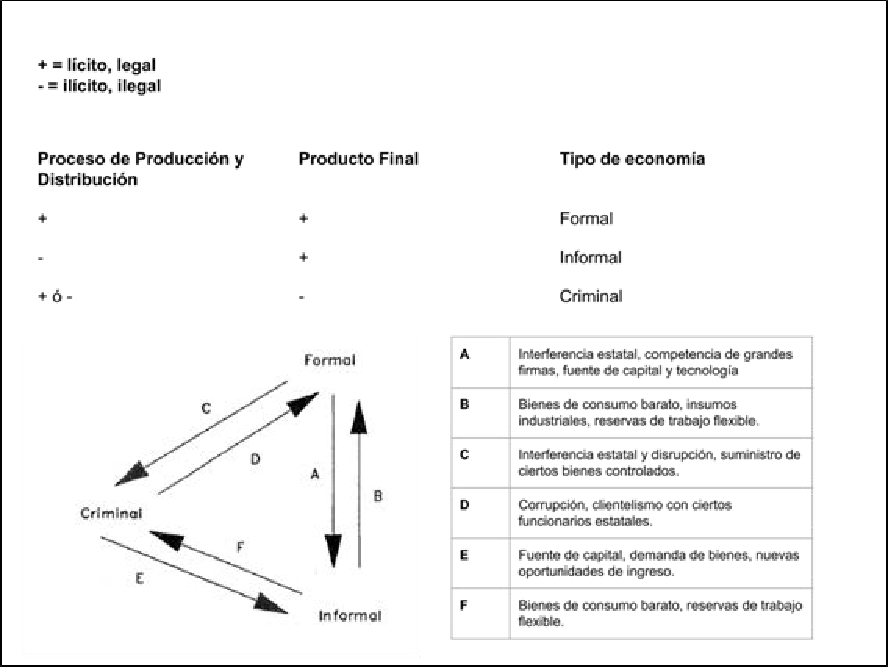
\includegraphics[width=4.16667in,height=\textheight]{Chapters/../Figures/portes_informal.pdf}

}

\end{figure}

\noindent \small Fuente: Portes et~al.
(\protect\hyperlink{ref-theinfo1989}{1989, p. 14}). Traducción propia
\normalsize

En la Figura~\ref{fig-esquema} podemos apreciar que existe tanto
cooperación como interferencia entre estas esferas. En primer lugar, la
economía formal genera interferencia con la economía informal y criminal
en tanto que la regulación estatal se encuentra vigilante del proceso de
producción y distribución. Asimismo, la competitividad de las empresas
dentro de esta economía en la mayoría de casos supera a la economía
informal en la calidad de los productos y/o servicios. En segundo lugar,
la economía informal suele suministrar bienes de consumo barato y mano
de obra en la medida que gran cantidad de procesos se tercerizan desde
la economía formal a la informal, dado que resulta conveniente la
flexibilidad de la mano de obra.

Por último, la economía criminal, al necesitar evadir a toda costa la
interferencia estatal, coopta a y corrompe funcionarios estatales para
poder operar de manera prolongada.

\hypertarget{causas-de-la-informalidad}{%
\section{Causas de la informalidad}\label{causas-de-la-informalidad}}

Existe debate acerca de las causas o al origen de la informalidad. Esto
ha llevado a que se generen corrientes que enfatizan cierto aspecto como
la causa principal que explica en mayor medida la informalidad.

\hypertarget{crisis-latinoamericana-en-la-duxe9cada-de-los-80s}{%
\subsection{Crisis latinoamericana en la década de los
80's}\label{crisis-latinoamericana-en-la-duxe9cada-de-los-80s}}

En América latina, la década de 1980 es conocida como la ``década
perdida'' por el estancamiento y retroceso económico en la región debido
al sobreendeudamiento internacional y la inflación interna. Como
consecuencia de esta crisis se pudo observar un aumento de la pobreza,
aumento en la desigualdad, caída salarial en el sector formal, desempleo
e informalidad del mercado laboral como nunca antes visto. Las causas de
esta catástrofe se pueden dividir en factores externos e internos.

Pérez-Sánchez (\protect\hyperlink{ref-puxe9rez-suxe1nchez1995}{1995});
Toussaint (\protect\hyperlink{ref-toussaint2004}{2004}) enumeran como
factores externos, la expansiva política monetaria de Estados Unidos y
el préstamo indiscriminado de capitales por parte de de los bancos
comerciales estadounidenses que operaban offshore. Después de la segunda
guerra mundial, Estados Unidos se había consolidado como la potencia
mundial que se encargaría del financiamiento de la reconstrucción de
Europa bajo el plan Marshall, abriendo el mercado estadounidense de
bienes de consumo al mundo. Esto llevó a un contexto de enorme liquidez
en una economía mundial dolarizada. En la década del 70, Estados Unidos
enfrenta una recesión económica asociada a la crisis del petróleo en
1973 que generó escasez del combustible y aumento del precio del barril
que se cuadruplicó. Este bloqueo de los pozos petrolíferos realizado por
la OPEC (Organización de Países Productores de Petróleo), junto con la
participación de Estados Unidos en la Guerra de Vietnam; llevó a que
Estados Unidos flexibilizara su regulación federal, lo que permitió que
muchos de sus bancos realizaran préstamos irresponsables con el objetivo
de generar mayor capital para el país.

Los grandes préstamos junto con el aumento de la tasa de intereses,
llevo a que muchos países latinoamericanos declaran la moratoria de pago
iniciando con México en 1982. Dos décadas de acumulación peligrosa de
deuda externa había llevado a que estos países no se encontraran en la
posibilidad de contribuir al pago de su deuda. Por lo que los bancos
transnacionales, con el peligro de quebrar, optaron por dejar de prestar
a los países de América Latina, contribuyendo a la crisis financiera en
la región.

Sumado a esto, como factores internos, podemos mencionar la necesidad de
endeudamiento para la industrialización de los países latinoamericanos.
Esta práctica no fue única en estos países. Japón y Corea del Sur habían
optado por una estrategia similiar lo que permitió que su economía se
diversificara y consolidaron una industria con valor agregado. Sin
embargo, en el caso latinoamericano, en el cual en su mayoría optaron
por la promoción de exportaciones y sustitución de importaciones, se
encontraron con algunas limitantes. En primer lugar, industrializar una
economía requiere de mano de obra calificada, transferencia de
tecnología, inversión en infraestructura, productividad de las grandes
empresas nacionales, entre otras cosas; las cuales toman décadas en
consolidar. A la par, los países latinoamericanos son faltantes crónicos
de divisas al exportar a bajo precio mayoritariamente materias primas
(sin valor agregado) e importar a alto precio manufacturas con valor
agregado; por lo que, al dejar de recibir préstamos de los bancos
comerciales se contribuyó a la recesión que sufriría la región.

La respuesta peruana al cobro de la deuda externa, fue encabezada
principalmente por el presidente Alan García (1985-1990) quien decretó
que solo se utilizaría el 10\% del ingreso por exportaciones para pagar
la deuda, a diferencia del 60\% del ingreso como se había realizado en
anteriores ocasiones. Además, rechazó la intermediación del FMI (Fondo
Monetario Internacional) frente a los bancos comerciales y, en cambio,
negociaría directamente con los bancos. Esta medida llevó a que el FMI
declarara al Perú como ``inelegible'' para préstamos ante la comunidad
internacional lo que acentuó la falta de inversión extranjera en el
país. La política intervencionista del ex-presidente García llevó a la
devaluación de la moneda local (Inti), dolarización de la economía
nacional, agotamiento de las reservas monetarias nacionales, colapso de
la Bolsa de Valores de Lima por estatización de la banca privada, entre
otros. De esta manera, se brindaron las condiciones para que frente a un
sector formal debilitado, con baja oferta laboral y bajos salarios, se
consolidara un sector informal con mayor flexibilidad laboral, menores
condiciones laborales, pero con ingresos variables.

\hypertarget{corriente-estructural}{%
\subsection{Corriente estructural}\label{corriente-estructural}}

Desde un punto de vista teórico, la corriente estructuralista
(\protect\hyperlink{ref-acemoglu2001}{Acemoglu, 2001};
\protect\hyperlink{ref-cacciamali1983}{Cacciamali, 1983};
\protect\hyperlink{ref-souza1980}{Souza, 1980};
\protect\hyperlink{ref-tokman1978}{Tokman, 1978}), predominante en los
años 80, considera que la principal causa de la permanencia y aumento
del sector informal es debido a que existe un sector de la economía
``moderno'' en la que se concentran los ``buenos empleos'', las
innovaciones tecnológicas, inversiones de capital extranjero, mano de
obra calificada y alta productividad, y que mantiene al margen a un
sector de la economía ``tradicional'' en el que se encuentran los
``malos'' empleos, trabajadores poco calificados y pagados con baja
productividad. Esta aproximación dualista de la economía considera que
es insuficiente la demanda laboral en el sector formal de la economía
para absorber a la masa de trabajadores y proveer empleo sobre todo poco
calificados por lo que las pequeñas empresas y empresas familiares optan
por la informalidad como una alternativa de supervivencia.

Desde esta aproximación, el sector informal tiene un desenvolvimiento
subordinado al desarrollo del sector formal, y emerge como resultado de
la falta de oportunidades laborales y económicas en una región o país.
La principal causa se asocia a factores económicos, falta de desarrollo
productivo. Un aspecto positivo de este enfoque es que plantea una
interrelación entre el sector formal y el sector informal, cuentan con
vasos comunicantes y no son compartimentos estancos.

No obstante, esta perspectiva ha sido criticada por Carneiro
(\protect\hyperlink{ref-carneiro1997}{1997}) debido a que se ha podido
observar de que en zonas económicamente activas en donde hay creación de
empleo y fluidez de capital, el empleo informal crece con mayor rapidez
junto con el empleo formal.

En un estudio realizado en Brasil, Carneiro
(\protect\hyperlink{ref-carneiro1997}{1997}) demostró como en las
regiones en donde había mayor dinamismo económico y en las que el empleo
formal estaba creciendo, crecía también en mayor medida el empleo
informal que en otras regiones con menor crecimiento económico (p.~16).
El autor argumenta que este fenómeno podría deberse a la creciente
importancia del sector ``servicios'', y a una crisis de la regulación
estatal, es decir, la incapacidad del gobierno de intervenir en el
sistema productivo. Asimismo, Pinilla Cisneros
(\protect\hyperlink{ref-cosamaluxf3n2018}{Cosamalón, 2018}) afirma que
esta corriente no incorpora el papel del Estado como un actor decisivo
en la propagación del sector informal y tampoco consideraba la
subcontratación hacia el sector informal de las grandes empresas.

\hypertarget{corriente-neoliberal}{%
\subsection{Corriente neoliberal}\label{corriente-neoliberal}}

La corriente neoliberal (\protect\hyperlink{ref-beiner1989}{Beiner,
1989}; \protect\hyperlink{ref-belapatiuxf1o2017}{Belapatiño et~al.,
2017}; \protect\hyperlink{ref-cartaya1987}{Cartaya, 1987};
\protect\hyperlink{ref-desoto1987}{H. de Soto et~al., 1987}),
predominante en los años 90 junto con el auge político del
neoliberalismo, considera que la principal causa del sector informal es
la excesiva reglamentación estatal del mercado laboral y el costo de
transacción en las actividades económicas. De esta manera, la
legislación laboral directa o indirectamente desincentiva la
contratación formal en tanto que las leyes suelen ser rígidas y no
permiten la flexibilidad en la contratación y despido de personal para
superar las imperfecciones del mercado. Esto, sumado a la percepción de
que no representa ningún beneficio para la empresa tener trabajadores
formales vuelve poco atractivo el proceso de formalización, a falta de
incentivos fiscales, y genera a que se incurra y perdure en la
informalidad. En adición, H. de Soto et~al.
(\protect\hyperlink{ref-desoto1987}{1987}) plantea que los engorrosos
trámites burocráticos serían una barrera de ingreso por los sectores
acomodados para impedir que los trabajadores pobres accedan a los
beneficios sociales y servicios del Estado.

Esta corriente enfatiza que el sector informal no solo está conformado
por pequeños negocios, sino también medianos y grandes con alta
productividad, tecnología y salarios, pero que incurren en tener
trabajadores no registrados, autoempleados, trabajadores independientes
no cubiertos en el seguro social por conveniencia
(\protect\hyperlink{ref-belapatiuxf1o2017}{Belapatiño et~al., 2017}).

Un aspecto positivo de esta corriente es que permitió considerar, como
parte del sector informal, a las actividades legitimas llevadas a cabo
por compañías formales que por múltiples razones eligen mantener una
parte de sus operaciones en la informalidad con trabajadores no
registrados. Esto, más adelante, fue catalogado como ``empleo informal
en el sector formal'' (\protect\hyperlink{ref-inei2020}{INEI, 2020}).
Asimismo, recuperó el papel de la decisión de los actores que antes eran
entendidos como víctimas pasivas de causas estructurales y había poco
que podían hacer para escapar de la situación de informalidad.

No obstante, esta perspectiva ha sido criticada por distintos autores
(\protect\hyperlink{ref-cosamaluxf3n2018}{Cosamalón, 2018};
\protect\hyperlink{ref-theinfo1989}{Portes et~al., 1989}) dado que
romantiza el sector informal peruano, ensalzan la informalidad como
reafirmación del espíritu empresarial en América Latina y promueven el
camino informal como una solución generalizada a las crisis económicas
de los países en que el sector tiene gran influencia. En la medida en
que se concentran en el proceso de formalización y sus limitaciones, se
deja de lado o en segundo plano lo que significa ser ``formal'' en
términos de beneficios sociales y cobertura; lo cual, puede llegar a ser
una limitación al momento de plantear soluciones.

Por otro lado, esta corriente rara vez incluye en su análisis los
factores estructurales como el modelo de desarrollo o el desempeño
macroeconómico de un país. Asimismo, Cosamalón agrega que en muchas
ocasiones, principalmente en América Latina, la difusión del comercio
informal respondió principalmente a un repliegue del Estado y de sus
medios de coacción por crisis fiscal, alteración política, violencia
insurgente, entre otras, lo que permitió el surgimiento de actores que
rivalizaran con las autoridades sobre el control del espacio público
como fue el caso de Perú en los 80's
(\protect\hyperlink{ref-cosamaluxf3n2018}{2018, p. 5}).

\hypertarget{corriente-multicausal}{%
\subsection{Corriente multicausal}\label{corriente-multicausal}}

Durand (\protect\hyperlink{ref-durand2007}{2007}) comenta que la
economía informal ``está constituida por empresas y trabajadores que
operan en una zona institucional claroscura''. Por lo que su nivel de
transgresión a la norma es limitado en tanto que no han cometido un
delito lesivo a la propiedad y a la persona. En el caso peruano, la
informalidad se suele reproducir cuando, por ejemplo, un conjunto de
ambulantes empieza a frecuentar una zona urbano-marginal para la venta
de sus bienes y servicios. Luego de generarse una masa crítica, se
constituyen los mercados informales en ``zonas liberadas'' del control
del Estado.

De esta manera, se reconoce el papel del Estado de reglar, fiscalizar
(\emph{enforcement}) y de establecer los mecanismos hacia la formalidad,
pero que; sin embargo, con frecuencia carecen de la capacidad para
regular plenamente las actividades y derechos en las sociedades
(\protect\hyperlink{ref-cosamaluxf3n2018}{Cosamalón, 2018}).Si bien el
Estado conoce la ubicación de estos espacios informales (e.g el
principal local de Sunat se encuentra a 3 cuadras de varios centros
comerciales de softwares piratas), su intervención es esporádica o
muchas veces nulas dependiendo de múltiples causas como un desborde para
controlar la economía, coimas a los funcionarios, entre otros. Dentro
del régimen de la economía informal, los trabajadores no se encuentran
en una planilla, si algún derecho tienen, este se da por costumbre antes
que por ley (\protect\hyperlink{ref-durand2007}{Durand, 2007, p. 81}).

Asimismo, Céspedes Reynaga
(\protect\hyperlink{ref-cuxe9spedesreynaga2020}{2020}) argumenta que la
informalidad resulta en un mecanismo de suavización de la contracción
y/o expansión economía. Por ello, muchos trabajadores optarían por el
sector informal al ser menos costosos el riesgo de desempleo en épocas
de crecimiento económico.

\hypertarget{corriente-neoestructural}{%
\subsection{Corriente neoestructural}\label{corriente-neoestructural}}

Portes et~al. (\protect\hyperlink{ref-theinfo1989}{1989}) argumentan que
la informalidad laboral se debe principalmente al proceso de
reestructuración económica mundial a raíz de la crisis del petróleo en
1973. A partir de este acontecimiento, las empresas internacionales,
para ser más competitivas, recurren en mayor medida al trabajo intensivo
informal por lo que no solo les beneficia la permanencia del sector
informal sino también su crecimiento y robustez. Estas empresas, muchas
veces en la forma de ``maquiladoras'', empresas financiadas por capital
extranjero para importar, procesar materia prima y exportarla a los
mismos países con valor agregado, buscan tercerizar su producción en el
sector informal abaratando costos.

Esto se podría entender como un proceso de descentralización productiva
donde los sectores modernos globales subcontratan para realizar sus
actividades tanto a nivel nacional como internacional, reificando y
promoviendo que las pequeñas y medianas empresas tengan trabajadores sin
contrato laboral para reducir costos y operar con las tarifas más bajas.

Por otro lado, plantean una caracterización de la informalidad que
incluya la amplitud de casos posibles en este sector. En primer lugar,
mencionan que la informalidad es un componente integrado en las
economías nacionales. No se desarrolla de manera independiente a la
economía formal, sino que interactúan para satisfacerse mutuamente
(\protect\hyperlink{ref-theinfo1989}{1989, p. 26}).

En segundo lugar, los trabajadores de la economía informal laboran en
una condición degradada en términos de beneficios sociales (seguro
contra accidentes, fondo de pensiones, entre otros). A la par, es más
difícil establecerse como un colectivo de presión (e.g un sindicato)
dada la falta de estabilidad en su labor sin contratos que lo aten.

En tercer lugar, si bien los trabajadores informales son muchas veces
intervenidos por los efectivos policiales, la actividad informal se
desarrolla ampliamente bajo la tolerancia del gobierno ya sea para
evitar conflictos sociales o para establecer patronaje político.

\hypertarget{efectos-de-la-informalidad}{%
\section{Efectos de la informalidad}\label{efectos-de-la-informalidad}}

A diferencia de las causas, existe relativo consenso acerca de las
consecuencias que puede traer el sector informal para la economía, las
empresas y los trabajadores. Con respecto a la economía, se forma un
modelo descentralizado de organización económica que busca reducir los
costos de producción (\protect\hyperlink{ref-theinfo1989}{Portes et~al.,
1989}). Las conexiones y subcontratación hacia el sector informal
generan un aumento de microempresas con múltiples proveedores que
contribuyen una fracción de la producción total.

Cabe mencionar que la informalidad representa de por sí una menor
recaudación tributaria que representa un obstáculo para la provisión de
bienes y servicios públicos
(\protect\hyperlink{ref-belapatiuxf1o2017}{Belapatiño et~al., 2017}). El
impuesto a la renta no recaudado del sector informal podría haber sido
invertido en educación, salud, justicia, infraestructura, seguridad
ciudadana, entre otras. Este déficit en la recaudación de impuestos
resulta en una sobrecarga impositiva en el sector formal dado que se
trata de optimizar al máximo la recaudación en este sector y de esta
manera también se afecta la productividad y competitividad de las
actividades formales.

Con respecto a las empresas, la informalidad laboral reduce su
productividad en tanto que las condiciones precarias y el bajo
equipamiento con la que laburan sus trabajadores les impide rentabilizar
su productividad.

Con respecto a los trabajadores, se debilita el poder de lucha sindical
o la capacidad de exigir un cambio de los trabajadores que contribuyen
al sector informal dado que no existen mecanismos legales que garanticen
su permanencia en un oficio (\protect\hyperlink{ref-theinfo1989}{Portes
et~al., 1989}). En el sector informal abundan las relaciones de trabajo
inestables, temporales y esporádicas por lo que el trabajador informal
debe alinearse con las condiciones precarias de trabajo, los horarios
abusivos, entre otros, dado que siempre existe la posibilidad de ser
reemplazado por un ejército de desempleados dispuesto a someterse a esas
condiciones de trabajo. Asimismo, la informalidad tiende a trasladar los
costos de la producción a los trabajadores siendo cada vez más común los
talleres domiciliarios sustituyendo a las fábricas centralizadas.

\hypertarget{salidas-a-la-informalidad}{%
\section{Salidas a la informalidad}\label{salidas-a-la-informalidad}}

Belapatiño et~al. (\protect\hyperlink{ref-belapatiuxf1o2017}{2017})
sugiere que se modifique la normativa laboral para promover la
formalización de las empresas en términos de flexibilizar las relaciones
laborales. Es así como manifiesta la necesidad de facilitar la
contratación y el despido en una empresa formal para que el negocio
pueda superar situaciones adversas o inesperadas en la economía y el
mercado laboral como lo es la pandemia del COVID-19. Esto se puede ver
reflejado en un estudio realizado por Apoyo Consultoría en que se
muestra que 54\% de los empleadores entrevistados mencionó que su
principal tema de preocupación en materia laboral es la dificultad para
despedir trabajadores, 43\% comenta que es difícil gestionar los
recursos humanos en el marco de la fiscalización del Estado), 35\%
resalta el encarecimiento de mano de obra calificada.

Asimismo, se sugiere la simplificación de la reglamentación laboral para
reducir los trámites y el tiempo que toma para que una empresa formal se
pueda constituir (\protect\hyperlink{ref-belapatiuxf1o2017}{Belapatiño
et~al., 2017}). Inclusive plantear incentivos tributarios para que las
empresas registren a sus trabajadores y mantengan en regla sus archivos
contables.

Otra posibilidad que plantean diferentes autores
(\protect\hyperlink{ref-belapatiuxf1o2017}{Belapatiño et~al., 2017}) es
la implementación de salarios mínimos diferenciados por el sector
productivo en el cual se labore.

Existen salidas a la informalidad que hacen énfasis en mejorar la
productividad de los trabajadores a través de condiciones estructurales.
Céspedes Reynaga (\protect\hyperlink{ref-cuxe9spedesreynaga2020}{2020})
argumenta que, si bien el crecimiento económico y la productividad del
sector formal empuja la generación de empleo hacia la formalidad, el
efecto es mínimo por lo que se requiere de otras soluciones más
directas. Entre estas se podrían considerar políticas activas que
mejoren el nivel educativo, la calidad y cobertura de los servicios de
salud, la infraestructura vial, entre otros. Este aumento de la
productividad debe ser focalizado; ya que, no todos los sectores de la
economía operan al mismo nivel de productividad.

Según el INEI (\protect\hyperlink{ref-belapatiuxf1o2017}{Belapatiño
et~al., 2017}), el sector ``minero e hidrocarburos'' es 40 veces más
productivo que el ``agropecuario y pesca''. Asimismo, el sector
``servicios y comercio'', donde se ubica la mayor parte de la PEA
ocupada, es 6 veces más productivo que el ``agropecuario y pesca''. De
esta manera, se muestra que uno de los sectores en que es más urgente
intervenir para reducir la informalidad es el sector ``servicios y
comercio'' por su predominancia en la economía peruana. Ahora bien,
Beteta (\protect\hyperlink{ref-beteta2020}{2020}) afirma que en el 2019,
en América Latina, la mayoría de empleos nuevos se generaron en los
sectores de comercio de los restaurantes y hoteles caracterizado por la
concentración de empleo informal; sin embargo, fue justamente este
sector el cual fue el más impactado por la pandemia del COVID-19 que
dispuso a los gobiernos a aplicar cuarentenas parciales o totales, se
limitaron los aforos, el poder de compra de los trabajadores se estancó,
entre otras barreras que experimentaron estas empresas ya sea formales
como informales.

\hypertarget{caso-internacional}{%
\section{Caso internacional}\label{caso-internacional}}

La Organización Internacional del Trabajo entiende al ``sector
informal'' como el universo de establecimientos de las unidades de
producción dedicadas a la producción de bienes y/o servicios con la
finalidad de crear empleos y generar ingresos para las personas
involucradas en la actividad económica
(\protect\hyperlink{ref-oit2002}{OIT, 2002}). Las unidades de producción
en la economía informal presentan principalmente los rasgos de las
empresas de hogares, es decir, que las obligaciones de la empresa no
recaen en sí misma sino en sus propietarios, y es a nombre ellos que se
efectúan las transacciones con otras unidades productivas. Es por ello
por lo que, muchas veces, los gastos de la empresa se encuentran
indistinguibles de los gastos de las familias involucradas en la
producción. La OIT menciona que estas empresas de empleadores informales
se caracterizan por tener una baja cantidad de empleados, estos
empleados suelen no estar oficialmente registrados, entre otros.

Por otro lado, el ``empleo informal'' se entiende como el número total
de empleos informales de los trabajadores involucrados en la economía
(\protect\hyperlink{ref-oit2002}{OIT, 2002}). Dentro de esta categoría
se encuentran, por ejemplo, los trabajadores y empleadores por cuenta
propia (independientes) dueños de sus propias empresas del sector
informal, trabajadores familiares auxiliares ya sean partícipes del
sector formal e informal, miembros de cooperativas de productores
informales (no constituidas formalmente ante entidades legales),
asalariados (no sujetos a la legislación laboral nacional) que tienen
empleos informales, entre otros.

\hypertarget{caso-peruano}{%
\section{Caso peruano}\label{caso-peruano}}

Luego de la aplicación del paquete de medidas de reestructuración
económica ``fujishock'' con la subida a la presidencia de Alberto
Fujimori, junto con la nueva constitución de 1993, se puede observar una
liberalización del mercado laboral, lo cual, en parte, volvía más
vulnerable a la economía peruana a las crisis financieras. De esta
manera, en la década del 90, el Perú retomó su cercanía con el Fondo
Monetario Internacional (FMI) y con los capitales extranjeros
priorizando un modelo económico extractivista de los recursos minerales
e hidrocarburos por parte de grandes empresas transnacionales. Esta
economía de enclave suele ser baja en generación de trabajo mientras que
sus actividades productivas no se integran al mercado local.

Por otro lado, como parte de las medidas neoliberales en el fujimorismo,
se limitaron las funciones intervencionistas del Estado en el mercado
laboral por lo que el crecimiento del sector formal se determinó bajo
las leyes de la oferta y demanda, y en relación, principalmente, con los
capitales extranjeros.

Dicho esto, un exponente peruano de los estudios sobre el sector
informal y que fue asesor cercano de Fujimori, fue Hernando de Soto,
quien fue un autor influyente, principalmente en los 90's, llegando a
tener un impacto directo en diferentes políticas públicas. Muchas de sus
tesis acerca de la informalidad fueron aplicadas en la Comisión de
Formalización de la Propiedad Informal (COFOPRI). H. de Soto et~al.
(\protect\hyperlink{ref-desoto1987}{1987}) consideraba que los elevados
costos de la formalidad llevaban a al auge de la construcción informal y
por consecuencia a las barriadas, las cuales eran vistas como un proceso
autogestionario frente a la ineficiencia estatal. Por lo que, resultaba
lógico que si el Estado reconocía la formalidad del terreno ocupado de
manera informal podía tener una influencia positiva en el tipo de
actividades laborales que se realizaban en estos espacios mientras que
se recaudaban impuestos de estos terrenos a la par que los autoempleados
se convertían propietarios de sus medios de producción abalados por el
Estado y así superar la pobreza urbana.

De esta manera, en el marco de la política de la titulación masiva por
parte del gobierno fujimorista se crea COFOPRI en 1996, con asesoría de
H. de Soto y el financiamiento del Banco Mundial. Sin embargo, en la
práctica este organismo se dedicó únicamente a la entrega de títulos de
dominio y no se reparó en la calidad de la vivienda y del espacio en que
se construía (\protect\hyperlink{ref-torres2019}{Torres \& Ruiz-Tagle,
2019}).

Esquivel (\protect\hyperlink{ref-esquivel2011}{2011}) argumenta que en
términos de entregar títulos de propiedad la comisión fue efectiva; pero
que, si observamos los objetivos que realmente buscaba cambiar se
evidencia que la inversión realizada en la propiedad posterior a la
entrega fue mínima, el acceso a servicios básicos fue reducido, la
obtención de préstamos bancarios fue principalmente estatal y rara vez
de entidades privadas, entre otros
(\protect\hyperlink{ref-esquivel2011}{2011, p. 2}). Asimismo, la
política pública de formalización urbana con COFOPRI ha traído como
consecuencia el incremento de tráfico de terrenos dada la simplicidad de
trámites en la obtención de títulos de dominio inclusive desconociendo a
dueños anteriores. De esta manera, resultó insuficiente la explicación
de que la informalidad se debía principalmente a la falta de extensión
del crédito y las hipotecas dado que en la práctica requería mucho más
que eso.

Ahora bien, en concordancia con las directrices planteadas por la OIT,
el Instituto Nacional de Estadística e Informática (INEI, Perú) ha
adoptado como parte del estudio y monitoreo de la economía informal la
dualidad entre el sector y el empleo informales.

El primero, según el INEI, refiere a las ``empresas de hogares (unidades
productivas no constituidas en sociedad, excluyendo las cuasisociedades)
que no están registradas en la administración tributaria (SUNAT)''
(\protect\hyperlink{ref-inei2020}{INEI, 2020}). En tanto que la unidad
de estudio son las unidades productivas, se busca recopilar esta
información a través de una ``Encuesta de establecimientos''
principalmente.

El segundo, se encuentra enmarcado en el total de empleos que cumplen
con alguna de las siguientes condiciones: a) los patronos y cuenta
propia cuya unidad productiva pertenece al sector informal, b)
asalariados sin seguridad social financiada por su empleador, c) los
trabajadores familiares no remunerados que laboran la unidad productiva.
En tanto que la unidad de estudio son las unidades productivas, se busca
recopilar esta información a través de una ``Encuesta de
establecimientos'' principalmente. Esta distinción nos permite apreciar
los empleos informales que se encuentran fuera del sector informal
considerando a aquellos asalariados del sector ``formal'' con empleo
informal.

\begin{figure}

\caption{\label{fig-pea}Clasificación de la PEA informal}

{\centering 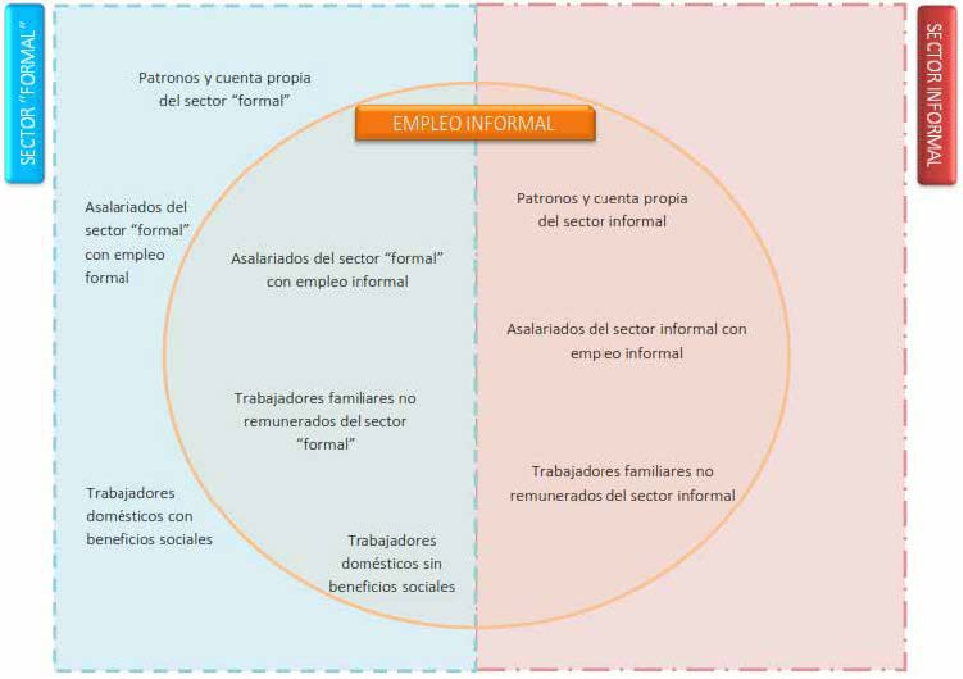
\includegraphics[width=4.16667in,height=\textheight]{Chapters/../Figures/pea_informal1.pdf}

}

\end{figure}

\noindent \small Fuente: Instituto Nacional de Estadística e Informática
-- 2017: ``Producción y Empleo Informal en el Perú 2017-2016''; en
Mantilla (\protect\hyperlink{ref-mantilla2021}{2021}) \normalsize

Cosamalón (\protect\hyperlink{ref-cosamaluxf3n2018}{2018}) destaca,
desde una aproximación cualitativa a la informalidad en el Perú, de que
una de las figuras centrales en el sector informal es el revendedor
ambulatorio que no solo vende un stock de productos en la calle para
poder sobrevivir, sino que es parte de un proceso de reconfiguración de
la economía mundial.

Sobre el caso peruano, Cosamalón tiene especial interés en las formas de
supervivencia que se utilizaron en las calles, a lo que comúnmente se
denomina ``trabajo callejero'' pero sin desmerecer la memoria y dignidad
de las personas que buscan salir adelante por sus propios medios. La
figura del vendedor ambulante se encuentra bastante presente en el Perú
donde la disminución del salario real, en la década de 1990, deprimió la
capacidad de consumo de los diferentes estratos sociales creando una
demanda por el precio más bajo. Plantea, además, que resulta crucial el
rol del ``capital social'' para comprender las dinámicas del sector
informal urbano y en especial al fenómeno ambulatorio. Como hemos
mencionado anteriormente, al no contar con mecanismos de protección
social públicos, los trabajadores informales crean sus propias redes de
apoyo mutuo las cuales requieren inversión y mantenimiento.

Estudios realizados en el Perú
(\protect\hyperlink{ref-cuxe9spedesreynaga2020}{Céspedes Reynaga, 2020};
\protect\hyperlink{ref-chacaltana2016}{Chacaltana, 2016}) destacan lo
siguiente, utilizando bases de datos como la Encuesta Nacional de
Hogares (ENAHO) y la Encuesta Permanente de Empleo (EPE): en primer
lugar, la informalidad urbana promedio varía entre 53\% y 75\%
dependiendo de la definición operativa que se utilice y sin considerar
tiempos de crisis. En segundo lugar, la informalidad laboral entre 2004
y 2014 se redujo entre -2,4\% y -0.5\%. Esta reducción ha venido a la
par con un incremento de la tasa de empleo formal principalmente entre
los trabajadores asalariados que entre 2002 y 2012 pasó del 41\% al 50\%
(\protect\hyperlink{ref-chacaltana2016}{Chacaltana, 2016, p. 52}).

Rodríguez \& Higa (\protect\hyperlink{ref-rodruxedguez2010}{2010})
confirman, utilizando la ENAHO, que el denominado ``sector informal'' ha
tenido una lenta tendencia a la baja independientemente que definición
se utilice en la década del 2000, lo cual se verá que difiere de la
situación actual. Asimismo, muestran que la conducción de las unidades
de producción informales suele estar a cargo de las mujeres. Esta
tendencia ha ido en aumento constituyéndose en un 56,2\% de mujeres en
el 2008 (p.19). Por otro lado, en relación con las unidades productivas,
observan que el 55\% no cuentan con local fijo, entre 10\% y 20\%
cuentan con servicios de agua y desagüe en su local, aunque poco más de
la mitad cuenta con electricidad en su local de trabajo, cerca del 3\%
cuenta con telefonía o internet.

Más aún, Higa et~al. (\protect\hyperlink{ref-higa2021}{2021}) señalan
que durante el primer año de la pandemia, los más afectados dentro de la
fuerza laboral fueron los trabajadores poco calificados, los
trabajadores de servicios, los jóvenes, mujeres (sobre todo con hijos
menores), y minorías étnicas. Asimismo, se ha incrementado la brecha
entre los trabajadores con educación y los que cuentan con menor
educación formal. Esta brecha se incrementó al inicio de la pandemia y
ha persistido más de un año después. Este estudio publicado en 2021 se
cuestiona si la brecha será superada una vez la pandemia esté bajo
control.

Si consideramos las principales características estructurales de la
informalidad laboral en el Perú, distintos autores
(\protect\hyperlink{ref-barco2010}{Barco \& Vargas, 2010};
\protect\hyperlink{ref-cuxe9spedesreynaga2020}{Céspedes Reynaga, 2020};
\protect\hyperlink{ref-chacaltana2016}{Chacaltana, 2016};
\protect\hyperlink{ref-rodruxedguez2010}{Rodríguez \& Higa, 2010})
mencionan las siguientes:

\begin{itemize}
\item
  La informalidad laboral usualmente cuenta con trabajadores con pocos
  años de educación.
\item
  Cuenta con trabajadores con pocas habilidades laborales.
\item
  Cuenta con trabajadores con bajo nivel educativo.
\item
  Laboran en micro y pequeñas empresas.
\item
  Afecta mayormente a las mujeres.
\item
  Afecta mayormente a los empleos no asalariados.
\item
  Afecta principalmente a trabajadores jóvenes y adultos mayores.
\item
  Es mayor en áreas urbanas fuera de Lima Metropolitana.
\item
  Predomina en el sector de comercio, construcción y en actividades
  primarias.
\end{itemize}

Hemos visto que no existe una definición conceptual singular de la
informalidad laboral, en parte, por el distinto énfasis que se le otorga
a la diversos elementos que constituyen la informalidad. Del mismo modo,
Céspedes Reynaga (\protect\hyperlink{ref-cuxe9spedesreynaga2020}{2020})
considera que existen múltiples definiciones operativas al momento de
querer medir el fenómeno en cuestión, para identificar a los
trabajadores informales en una economía.

El INEI identifica a los trabajadores informales considerando la
diferencia entre el sector informal y el sector formal establecido por
la OIT en su XIII Conferencia Internacional de Estadísticas de Trabajo o
CIET por sus iniciales
(\protect\hyperlink{ref-cuxe9spedesreynaga2020}{Céspedes Reynaga,
2020}). Asimismo,

\begin{quote}
``considera como trabajador informal a los patronos y por cuenta propia
cuya unidad productiva pertenece al sector informal, los asalariados
(del sector formal) sin seguridad social financiada por su empleador, y
los trabajadores familiares no remunerados, independientemente de la
naturaleza formal o informal de la unidad productiva donde trabaja''
(Céspedes Reynaga, 2020).
\end{quote}

Céspedes Reynaga afirma que, para cubrir los diferentes casos, se
plantean los siguientes tipos de definiciones operacionales para
identificar trabajadores informales dependientes asalariados y para los
trabajadores del hogar:

\begin{itemize}
\item
  Informalidad por ingresos: incluye a los trabajadores informales que
  perciben un salario mínimo por hora menor al establecido por la ley
  (actualmente s/.1025).
\item
  Informalidad por afiliación al sistema de pensiones: incluye a los
  trabajadores informales que declaran no estar afiliados a ningún
  sistema de pensiones (público o privado).
\item
  Informalidad por libros contables: incluye a los trabajadores
  informales que mencionaron conocer que la empresa donde labora no
  lleva libros contables.
\item
  Informalidad por personería jurídica: trabajadores informales que
  trabajan en empresas sin personería jurídica.
\item
  Informalidad por contrato: trabajadores informales que laboran sin
  ningún tipo de contrato.
\item
  Informalidad por impuestos laborales: trabajadores informales que
  mencionaron no pagar ningún descuento laboral.
\end{itemize}

Considerar los distintos tipos de informalidad de manera independiente y
en su conjunto es útil cuando no se cuenta con información acerca de
alguno de los indicadores.

\hypertarget{suxedntesis}{%
\section{Síntesis}\label{suxedntesis}}

Luego de lo expuesto, podemos concluir que siendo la informalidad
laboral una temática desarrollada a finales del siglo pasado, una gran
cantidad de estudios se limitan a estudiarla como un todo unificado
(cantidad de personas involucradas, producción económica anual, etc.) y
no predominan los estudios que se concentren en la diferenciación y
variedad de casos que existen dentro de la informalidad. Este es un
vacío que la presente investigación busca compensar.

\bookmarksetup{startatroot}

\hypertarget{sec-marco}{%
\chapter{Marco Teórico}\label{sec-marco}}

Para este estudio, me basaré en las definiciones planteadas por el INEI,
que a su vez se apoyan en los lineamientos sugeridos por la OIT, en
tanto que utilizo como fuente de información las bases de datos
recopiladas en la Encuesta Nacional de Hogares (ENAHO). En adición, se
acota la población de estudio a los trabajadores ubicados en las urbes
del Perú dado que la experiencia de la informalidad laboral difiere
tanto en el ámbito rural como en el urbano, lo cual tiene implicancias
en el estudio de las condiciones de vida.

Para identificar a los trabajadores informales, el INEI selecciona a la
Población en Edad de Trabajar (PET) la cual consiste en las personas de
14 años a más y que, a su vez, se subdivide en Población Económicamente
Activa (PEA) y Población Económica Inactiva (PEI). La primera, refiere a
aquellos que en la semana de referencia consultada en la encuesta se
encontraban trabajando, no trabajaban, pero tenían trabajo, o se
encontraban buscando activamente un trabajo. La segunda, refiere a
aquellos que no se encontraban buscando un trabajo a la fecha.

Dentro de la PEA, se considera como ``ocupados'' a todos aquellos que
estuvieron participando en alguna actividad económica; los trabajadores
dependientes que aunque tuvieron un empleo fijo no trabajaron la semana
anterior por motivo de vacaciones, huelga, licencia por enfermedad,
licencia de maternidad, entre otras, todas estas pagadas; los
trabajadores independientes que estuvieron ausentes en sus trabajos pero
la empresa o negocio continúa funcionando; los trabajadores que no
teniendo un empleo constante realizaron un oficio por al menos una hora
y fueron remunerados con dinero y/o especie; por último, los
trabajadores familiares no remunerados que trabajaron 25 horas o más,
practicantes, fuerzas armadas y policiales.

Como hemos visto anteriormente, el estudio de la informalidad se puede
abordar desde el punto de vista de las unidades productivas fuera de los
registros públicos (sector informal) o de la fuerza laboral (empleo
informal) la cual puede trabajar sin un contrato formal, sin beneficios
sociales, en condiciones de trabajo deplorables, entre otras. En la
medida en que nos centraremos en estudiar las condiciones de vida,
representadas en el ingreso mensual, optaremos por centrarnos en el
``empleo informal'' y en el ``empleo formal''.

\hypertarget{empleo-informal}{%
\section{Empleo informal}\label{empleo-informal}}

El empleo informal refiere al total de empleos dentro de la Población
Económicamente Activa Ocupada (PEAO) que cumplen alguna de las
siguientes condiciones, según la categoría de ocupación del trabajador:

\begin{enumerate}
\def\labelenumi{\roman{enumi})}
\tightlist
\item
  Los patronos y cuenta propia cuya unidad productiva pertenece al
  sector informal.
\item
  Los asalariados sin seguridad social financiada por su empleador.
\item
  Los trabajadores familiares no remunerados, independientemente de la
  naturaleza formal o informal de la unidad productiva donde labora.
\end{enumerate}

Dentro del empleo informal se puede distinguir entre dos grupos siendo
los que trabajan de manera independiente, y los que se desenvuelven
dentro unidades productivas: empleados, empleadores, obreros y
trabajadores familiares no remunerados
(\protect\hyperlink{ref-cuxe9spedesreynaga2020}{Céspedes Reynaga, 2020};
\protect\hyperlink{ref-sanchuxe9zvillagomez2019}{Sanchéz Villagomez \&
Chafloque Céspedes, 2019}). Asimismo, como hemos mencionados
anteriormente, la barrera entre el sector formal y el informal es
porosa, y fluctúan los empleos informales entre ambos sectores con
condiciones laborales muy distintas; no obstante, predominan las
condiciones precarias.

\hypertarget{empleo-formal}{%
\section{Empleo formal}\label{empleo-formal}}

Comprende a los patronos y cuenta propia, asalariados y trabajadores
domésticos con beneficios sociales del sector formal
(\protect\hyperlink{ref-inei2021}{INEI, 2021}).

\hypertarget{condiciones-de-vida}{%
\section{Condiciones de vida}\label{condiciones-de-vida}}

Entenderemos como ``condiciones de vida'' al ingreso neto que tienen los
hogares que les permiten satisfacer sus necesidades a través de bienes
de consumo y servicios. Con el objetivo de observar el impacto directo
de la pandemia en las condiciones de vida de los trabajadores y sus
hogares, se ha priorizado como indicador el ingreso mensual proveniente
del trabajo. De esta manera, se considera el ingreso promedio
correspondiente a la PEA ocupada con ingresos mayores a cero y que
provienen de su actividad principal, secundaria, trabajo dependiente e
independiente, y puede llegar a ser monetario o no monetario (pago en
especias). Asimismo, se procesa esta variable para los residentes
habituales, ya sean miembros del hogar o no miembros, pero que
estuvieron presentes en el hogar en los últimos 30 días.

\hypertarget{nivel-de-pobreza}{%
\section{Nivel de pobreza}\label{nivel-de-pobreza}}

En 2010, la Comisión Consultiva para la Estimación de la Pobreza
(\protect\hyperlink{ref-inei2010}{INEI, 2010}) por encargo del INEI
mencionó, en función de los precios de la canasta de alimentos y la
remuneración mínima vital (RMV), que se podría definir los hogares
pobres cuyos ingresos se encuentran alrededor de s/.178 y s/.385. Este
cálculo ha sido establecido, a su vez, considerando la comparabilidad
con encuestas de años anteriores.

\bookmarksetup{startatroot}

\hypertarget{sec-hipotesis}{%
\chapter{Hipótesis}\label{sec-hipotesis}}

A partir de la literatura expuesta, se muestra que la mayoría de la
población económicamente activa (PEA) se encuentra involucrada en el
empleo informal y que su reducción ha sido un proceso continuo,
progresivo, pero lento. Tomando en cuenta que el gobierno aplicó medidas
de restricción de la movilidad social de manera más estricta al inicio
de la pandemia para contener el virus dificultando que muchos negocios
informales pudieran conectar con la demanda a la cual satisfacían; y
que, a pesar de las medidas de restricción, los trabajadores, sobre todo
informales, continuaron en la medida de lo posible brindando sus bienes
y servicios dado que muchas su subsistencia depende de la ganancia
diaria.

En tal sentido nos planteamos las siguientes hipótesis:

\textbf{H1.} La pandemia ha tenido como efecto un incremento de la PEA
ocupada en situación de informalidad.

\textbf{H2.} Este incremento ha sido mayor en las zonas y grupos
sociales más vulnerables, especialmente: A.

\begin{enumerate}
\def\labelenumi{\roman{enumi}.}
\item
  Zonas urbanas de la Sierra y de la Selva
\item
  Ciudades de pequeña y mediana escala
\item
  Entre los jóvenes y mujeres
\item
  Entre los trabajadores con menor nivel educativo
\end{enumerate}

\textbf{H3.} La pandemia ha tenido un efecto negativo en el ingreso neto
de los trabajadores en general, pero este efecto ha sido mayor en el
caso de los trabajadores informales

\textbf{H4.} Este deterioro será mayor en los grupos más vulnerables
como jóvenes, y personas con menor nivel educativo.

\bookmarksetup{startatroot}

\hypertarget{sec-metod}{%
\chapter{Metodología}\label{sec-metod}}

El presente estudio cuenta con una metodología cuantitativa de corte
longitudinal considerando los años 2019-2021 sobre la base de la base de
datos de la Encuesta Nacional de Hogares (ENAHO) llevado a cabo por el
INEI. En primer lugar, se realizará un análisis descriptivo de la PEA
ocupada urbana en busca de diferencias según las siguientes variables
independientes:

\begin{itemize}
\item
  Dominio geográfico
\item
  Estrato geográfico
\item
  Sexo
\item
  Grupos de edad
\item
  Nivel educativo alcanzado
\item
  Categoría ocupacional
\item
  Condición de pobreza
\end{itemize}

En segundo lugar, se evalúan los cambios en los niveles de informalidad
del empleo del trabajador (variable dependiente -- V.D) según las
variables independientes antes mencionadas.

En tercer lugar, se revisan los cambios en el ingreso promedio por
trabajo mensual en soles de la PEA ocupada urbana (V.D) considerando la
condición de informalidad del trabajador (V.D) según las variables
independientes antes mencionadas. Cabe mencionar que se ha utilizado el
valor monetario deflactado e imputado de los ingresos promedios lo que
permite que los datos se encuentren anualizados, ajustado por el
promedio mensual del índice de precios al consumidor (IPC), y se filtran
o se imputan los valores perdidos.

Con respecto a la base de datos utilizada, para motivos del estudio se
emplea la Encuesta Nacional de Hogares (ENAHO), específicamente
orientado a los hogares en el área urbana, en los 24 departamentos del
país y en la Provincia Constitucional del Callao. Dentro de esta
encuesta, se utiliza particularmente el módulo 5: Empleo e Ingreso el
cual se centra en recopilar información sobre las condiciones laborales,
número de horas trabajadas, ingresos y gastos, condición de formalidad,
entre otros. La ENAHO, al ser una encuesta basada en las personas que
conforman el hogar, requiere que se filtre a aquellas personas que no
forman parte del hogar y/o que no residen más de 30 días en el hogar.
Esto con la finalidad de poder realizar los cálculos en función del
mercado laboral.

Es así como para el año 2019 contamos con una base de datos de 39 141
trabajadores urbanos ocupados; para el 2020, con 31 675; y para el 2021,
con 36 203. Para la construcción de la base de datos en cuestión y los
cálculos estadísticos, se utilizó el lenguaje de programación R el cual
permite manipular bases de datos con rigurosidad científica. Para
observar las diferencias entre la Selva Alta y Selva Baja, se recodificó
la variable ``Dominio Geográfico'' utilizando la variable ``Altitud''
presente en el módulo 1: Características de la Vivienda y del Hogar. La
sintaxis elaborada se adjunta en los anexos. Dado que nos encontramos
con una muestra de carácter grande, se considerará como significativo la
variación porcentual alrededor de 2\%.

\bookmarksetup{startatroot}

\hypertarget{sec-resultados}{%
\chapter{Resultados}\label{sec-resultados}}

\hypertarget{anuxe1lisis-de-la-pea-ocupada-urbana}{%
\section{Análisis de la PEA ocupada
urbana}\label{anuxe1lisis-de-la-pea-ocupada-urbana}}

Durante los años 2019 y 2021, la PEA experimentó cambios atípicos en
comparación a años pasados. Desde 2015, la PEA había variado entre 2 y 4
puntos porcentuales hacia el alza
(\protect\hyperlink{ref-inei2021}{INEI, 2021}). Sin embargo, durante el
periodo de estudio, vemos una reducción de la PEA ocupada del 10\% y un
aumento de la PEA desocupada en 3\% hacia 2020. A esta caída a inicios
de la pandemia le sigue una recuperación parcial en 2021 que, si bien es
prometedora, no se equipara a los niveles prepandemia.

\begin{figure}

\caption{\label{fig-pea}Características de la PEA urbana entre 2019 y
2021}

{\centering 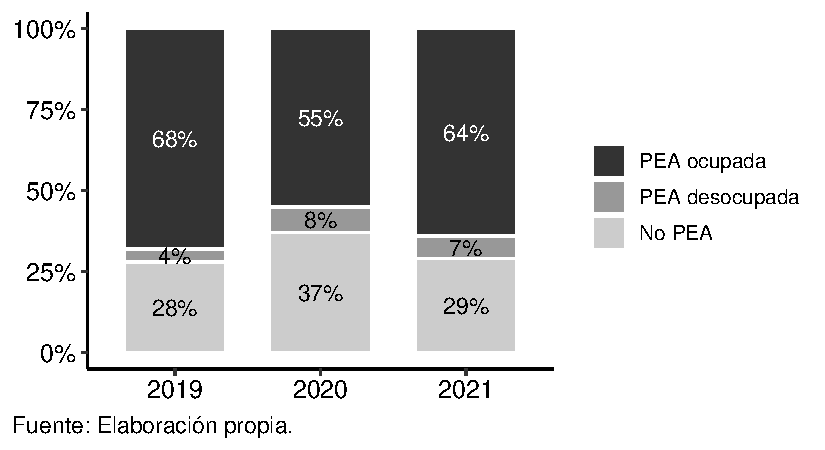
\includegraphics{Chapters/resultados_files/figure-pdf/fig-pea-1.pdf}

}

\end{figure}

\noindent \small Fuente: Elaboración propia. \normalsize

La Tabla~\ref{tbl-peadomes} muestra cómo se experimentó, en el ámbito
urbano, la caída de la PEA ocupada en 2020. Cerca a 2 millones de
empleos se perdieron en el ámbito urbano en 2020. Solo en Lima
Metropolitana se perdieron 150 mil empleos respecto del 2019 siendo la
región más afectada. Se puede observar que la recuperación hacia el 2021
ha sido sostenida, incluso destaca la Selva y el Sur (Costa y Sierra)
los cuales han excedido los niveles de empleo prepandemia mostrando una
mejor recuperación en líneas generales.

Por otro lado, si bien las ciudades con 500 000 habitantes a más fueron
las que más empleos perdieron, alrededor de un millón de empleos, las
ciudades intermedias de 50 a 100 mil habitantes fueron las que
proporcionalmente perdieron más empleos con cerca de 22\% de empleos
perdidos en 2020.

\hypertarget{tbl-peadomes}{}
\begin{table}[H]
\caption{\label{tbl-peadomes}Características de la PEA ocupada urbana según dominio y estrato entre
2019 y 2021 (porcentajes verticales) }\tabularnewline

\centering\begingroup\fontsize{10}{12}\selectfont

\begin{tabular}{cccc}
\toprule
\multicolumn{1}{c}{ } & \multicolumn{1}{c}{\textbf{2019}} & \multicolumn{1}{c}{\textbf{2020}} & \multicolumn{1}{c}{\textbf{2021}} \\
\cmidrule(l{3pt}r{3pt}){2-2} \cmidrule(l{3pt}r{3pt}){3-3} \cmidrule(l{3pt}r{3pt}){4-4}
\textbf{Variable} & Total en miles (\%) & Total en miles (\%) & Total en miles (\%)\\
\midrule
\cellcolor{gray!6}{\textbf{Nacional}} & \cellcolor{gray!6}{19,747 (100.00\%)} & \cellcolor{gray!6}{20,153 (100.00\%)} & \cellcolor{gray!6}{20,558 (100.00\%)}\\
\textbf{Dominio Geográfico} &  &  & \\
\cellcolor{gray!6}{Costa Norte} & \cellcolor{gray!6}{3,285 (16.64\%)} & \cellcolor{gray!6}{3,349 (16.62\%)} & \cellcolor{gray!6}{3,406 (16.57\%)}\\
Costa Centro & 1,537 (7.78\%) & 1,563 (7.76\%) & 1,585 (7.71\%)\\
\cellcolor{gray!6}{Costa Sur} & \cellcolor{gray!6}{466 (2.36\%)} & \cellcolor{gray!6}{468 (2.32\%)} & \cellcolor{gray!6}{481 (2.34\%)}\\
\addlinespace
Sierra Norte & 469 (2.38\%) & 479 (2.38\%) & 517 (2.51\%)\\
\cellcolor{gray!6}{Sierra Centro} & \cellcolor{gray!6}{1,497 (7.58\%)} & \cellcolor{gray!6}{1,531 (7.59\%)} & \cellcolor{gray!6}{1,554 (7.56\%)}\\
Sierra Sur & 2,215 (11.22\%) & 2,273 (11.28\%) & 2,326 (11.31\%)\\
\cellcolor{gray!6}{Selva Baja} & \cellcolor{gray!6}{1,613 (8.17\%)} & \cellcolor{gray!6}{1,663 (8.25\%)} & \cellcolor{gray!6}{1,653 (8.04\%)}\\
Selva Alta & 348 (1.76\%) & 360 (1.79\%) & 394 (1.92\%)\\
\addlinespace
\cellcolor{gray!6}{Lima Metropolitana} & \cellcolor{gray!6}{8,317 (42.12\%)} & \cellcolor{gray!6}{8,467 (42.01\%)} & \cellcolor{gray!6}{8,641 (42.03\%)}\\
\textbf{Ciudad (hab.)} &  &  & \\
\cellcolor{gray!6}{500 000 a más} & \cellcolor{gray!6}{9,718 (49.21\%)} & \cellcolor{gray!6}{9,926 (49.25\%)} & \cellcolor{gray!6}{10,259 (49.90\%)}\\
100 000 - 499 999 & 3,916 (19.83\%) & 3,808 (18.90\%) & 3,437 (16.72\%)\\
\cellcolor{gray!6}{50 000 - 99 999} & \cellcolor{gray!6}{1,131 (5.73\%)} & \cellcolor{gray!6}{1,071 (5.32\%)} & \cellcolor{gray!6}{1,152 (5.60\%)}\\
\addlinespace
20 000 - 49 999 & 1,718 (8.70\%) & 1,789 (8.88\%) & 1,816 (8.83\%)\\
\cellcolor{gray!6}{2 000 - 19 999} & \cellcolor{gray!6}{3,264 (16.53\%)} & \cellcolor{gray!6}{3,559 (17.66\%)} & \cellcolor{gray!6}{3,895 (18.94\%)}\\
\bottomrule
\end{tabular}
\endgroup{}
\end{table}

\noindent \small Fuente: Elaboración propia. \normalsize

Dentro de la PEA ocupada, se observa que más del 50\% de los
trabajadores son hombres y es una situación que se replica en el empleo
informal. Se tiene que 1 de cada 7 hombres trabajadores perdieron su
empleo, mientras que 1 de cada 5 mujeres trabajadoras perdieron su
empleo en 2020. Hacia el 2021, se observa que tanto hombres como mujeres
han tenido una recuperación en términos del tamaño de la fuerza laboral
siendo más lento en el caso de las mujeres. Además, la
Tabla~\ref{tbl-peasexeda} nos muestra una caída en el empleo
principalmente en la población de 25 a 44 años seguido de los
trabajadores de 14 a 24 años. De esta manera, hallamos que la pandemia
ha impactado principalmente a los trabajadores adultos jóvenes quienes
hacia finales de 2021 no habían restaurado los niveles prepandemia.
Asimismo, se observa de manera preocupante que los trabajadores mayores
de 60 años no han recuperado su situación prepandemia por lo que este
ajuste se está dando con lentitud.

\hypertarget{tbl-peasexeda}{}
\begin{table}[H]
\caption{\label{tbl-peasexeda}Características de la PEA ocupada urbana según sexo y grupo de edad
entre 2019 y 2021 (porcentajes verticales) }\tabularnewline

\centering\begingroup\fontsize{10}{12}\selectfont

\begin{tabular}{cccc}
\toprule
\multicolumn{1}{c}{ } & \multicolumn{1}{c}{\textbf{2019}} & \multicolumn{1}{c}{\textbf{2020}} & \multicolumn{1}{c}{\textbf{2021}} \\
\cmidrule(l{3pt}r{3pt}){2-2} \cmidrule(l{3pt}r{3pt}){3-3} \cmidrule(l{3pt}r{3pt}){4-4}
\textbf{Variable} & Total en miles (\%) & Total en miles (\%) & Total en miles (\%)\\
\midrule
\cellcolor{gray!6}{\textbf{Nacional}} & \cellcolor{gray!6}{13,360 (100.00\%)} & \cellcolor{gray!6}{11,172 (100.00\%)} & \cellcolor{gray!6}{13,229 (100.00\%)}\\
\textbf{Sexo} &  &  & \\
\cellcolor{gray!6}{Hombre} & \cellcolor{gray!6}{7,364 (55.12\%)} & \cellcolor{gray!6}{6,421 (57.48\%)} & \cellcolor{gray!6}{7,405 (55.97\%)}\\
Mujer & 5,996 (44.88\%) & 4,750 (42.52\%) & 5,825 (44.03\%)\\
\cellcolor{gray!6}{\textbf{Grupos de edad}} & \cellcolor{gray!6}{} & \cellcolor{gray!6}{} & \cellcolor{gray!6}{}\\
\addlinespace
14-24 & 2,095 (15.68\%) & 1,658 (14.84\%) & 2,079 (15.72\%)\\
\cellcolor{gray!6}{25-44} & \cellcolor{gray!6}{6,442 (48.21\%)} & \cellcolor{gray!6}{5,445 (48.74\%)} & \cellcolor{gray!6}{6,421 (48.53\%)}\\
45-59 & 3,318 (24.83\%) & 2,922 (26.15\%) & 3,400 (25.70\%)\\
\cellcolor{gray!6}{60-64} & \cellcolor{gray!6}{767 (5.74\%)} & \cellcolor{gray!6}{546 (4.89\%)} & \cellcolor{gray!6}{630 (4.76\%)}\\
65 a más & 739 (5.53\%) & 601 (5.38\%) & 699 (5.29\%)\\
\bottomrule
\end{tabular}
\endgroup{}
\end{table}

\noindent \small Fuente: Elaboración propia. \normalsize

En la Tabla~\ref{tbl-edpobre}, se observa que, entre 2019 y 2020, hubo
una reducción en 14\% de los trabajadores que tienen únicamente
educación secundaria o menos; no obstante, hacia 2021 se observa una
recuperación que llega a superar niveles prepandemia. En cambio, los
trabajadores con educación técnica o universitaria completa y más
tuvieron una reducción en 20\% de este sector con una recuperación mucho
más lenta, es decir, lo cual no se equipara a niveles prepandemia. De
esta manera, se encuentra que en un mercado laboral compuesto
principalmente por trabajadores con educación secundaria o menos, la
recuperación de este sector ha tenido mayor celeridad a diferencia de
los trabajadores que contaban con un título profesional, condición que
no necesariamente les aseguró un puesto de trabajo.

\hypertarget{tbl-edpobre}{}
\begin{table}[H]
\caption{\label{tbl-edpobre}Características de la PEA ocupada urbana según nivel educativo y pobreza
entre 2019 y 2021 (porcentajes verticales) }\tabularnewline

\centering\begingroup\fontsize{10}{12}\selectfont

\begin{tabular}{cccc}
\toprule
\multicolumn{1}{c}{ } & \multicolumn{1}{c}{\textbf{2019}} & \multicolumn{1}{c}{\textbf{2020}} & \multicolumn{1}{c}{\textbf{2021}} \\
\cmidrule(l{3pt}r{3pt}){2-2} \cmidrule(l{3pt}r{3pt}){3-3} \cmidrule(l{3pt}r{3pt}){4-4}
\textbf{Variable} & Total en miles (\%) & Total en miles (\%) & Total en miles (\%)\\
\midrule
\cellcolor{gray!6}{\textbf{Nacional}} & \cellcolor{gray!6}{13,360 (100.00\%)} & \cellcolor{gray!6}{11,172 (100.00\%)} & \cellcolor{gray!6}{13,229 (100.00\%)}\\
\textbf{Educación} &  &  & \\
\cellcolor{gray!6}{Sin nivel} & \cellcolor{gray!6}{225 (1.68\%)} & \cellcolor{gray!6}{171 (1.54\%)} & \cellcolor{gray!6}{205 (1.55\%)}\\
Secundaria incompleta o menos & 3,564 (26.68\%) & 3,060 (27.39\%) & 3,711 (28.05\%)\\
\cellcolor{gray!6}{Secundaria completa} & \cellcolor{gray!6}{4,177 (31.27\%)} & \cellcolor{gray!6}{3,622 (32.43\%)} & \cellcolor{gray!6}{4,434 (33.51\%)}\\
\addlinespace
Técnica incompleta & 787 (5.89\%) & 671 (6.00\%) & 823 (6.22\%)\\
\cellcolor{gray!6}{Técnica completa} & \cellcolor{gray!6}{1,687 (12.63\%)} & \cellcolor{gray!6}{1,376 (12.32\%)} & \cellcolor{gray!6}{1,542 (11.66\%)}\\
Universitaria incompleta & 1,004 (7.51\%) & 739 (6.62\%) & 897 (6.78\%)\\
\cellcolor{gray!6}{Universitaria completa} & \cellcolor{gray!6}{1,563 (11.70\%)} & \cellcolor{gray!6}{1,279 (11.45\%)} & \cellcolor{gray!6}{1,366 (10.32\%)}\\
Posgrado & 353 (2.64\%) & 253 (2.27\%) & 251 (1.90\%)\\
\addlinespace
\cellcolor{gray!6}{\textbf{Pobreza}} & \cellcolor{gray!6}{} & \cellcolor{gray!6}{} & \cellcolor{gray!6}{}\\
Pobre Extremo & 82 (0.62\%) & 196 (1.75\%) & 194 (1.46\%)\\
\cellcolor{gray!6}{Pobre No Extremo} & \cellcolor{gray!6}{1,465 (10.97\%)} & \cellcolor{gray!6}{1,984 (17.76\%)} & \cellcolor{gray!6}{2,128 (16.09\%)}\\
No Pobre & 11,813 (88.42\%) & 8,992 (80.49\%) & 10,907 (82.45\%)\\
\bottomrule
\end{tabular}
\endgroup{}
\end{table}

\noindent \small Fuente: Elaboración propia. \normalsize

Por otro lado, la pandemia ha afectado principalmente a los trabajadores
que se consideraban como no pobres en la medida en que hubo un descenso
de 2 millones de trabajadores no pobres y un aumento de los trabajadores
pobres no extremos y extremos. Sobre este punto, se observa que en 2020
los trabajadores pobres extremos se duplicaron llegando a representar el
1.75\% de la PEA ocupada urbana. Hacia el 2021, la presencia de
trabajadores pobres extremos no ha cambiado mucho manteniéndose
alrededor de 194 mil trabajadores.

Respecto a la posición ocupacional del trabajador, la
Tabla~\ref{tbl-peaocupinf} muestra que ha habido una mayor caída en los
trabajadores que se desempeñaban como empleados, cerca de un tercio de
ellos perdieron su empleo.

\hypertarget{tbl-peaocupinf}{}
\begin{table}[H]
\caption{\label{tbl-peaocupinf}Características de la PEA ocupada urbana según ocupación principal y
situación de informalidad entre 2019 y 2021 (porcentajes verticales) }\tabularnewline

\centering\begingroup\fontsize{10}{12}\selectfont

\begin{tabular}{cccc}
\toprule
\multicolumn{1}{c}{ } & \multicolumn{1}{c}{\textbf{2019}} & \multicolumn{1}{c}{\textbf{2020}} & \multicolumn{1}{c}{\textbf{2021}} \\
\cmidrule(l{3pt}r{3pt}){2-2} \cmidrule(l{3pt}r{3pt}){3-3} \cmidrule(l{3pt}r{3pt}){4-4}
\textbf{Variable} & Total en miles (\%) & Total en miles (\%) & Total en miles (\%)\\
\midrule
\cellcolor{gray!6}{\textbf{Nacional}} & \cellcolor{gray!6}{13,360 (100.00\%)} & \cellcolor{gray!6}{11,172 (100.00\%)} & \cellcolor{gray!6}{13,229 (100.00\%)}\\
\textbf{Ocupación principal} &  &  & \\
\cellcolor{gray!6}{Empleador} & \cellcolor{gray!6}{570 (4.27\%)} & \cellcolor{gray!6}{345 (3.09\%)} & \cellcolor{gray!6}{465 (3.51\%)}\\
Independiente & 4,563 (34.16\%) & 4,005 (35.85\%) & 4,767 (36.03\%)\\
\cellcolor{gray!6}{Empleado} & \cellcolor{gray!6}{4,065 (30.42\%)} & \cellcolor{gray!6}{3,056 (27.35\%)} & \cellcolor{gray!6}{3,479 (26.29\%)}\\
\addlinespace
Obrero & 2,968 (22.21\%) & 2,677 (23.96\%) & 3,327 (25.15\%)\\
\cellcolor{gray!6}{Familiar No Remunerado} & \cellcolor{gray!6}{774 (5.79\%)} & \cellcolor{gray!6}{830 (7.43\%)} & \cellcolor{gray!6}{833 (6.30\%)}\\
Trabajador del Hogar & 397 (2.97\%) & 231 (2.07\%) & 330 (2.50\%)\\
\cellcolor{gray!6}{Otro} & \cellcolor{gray!6}{23 (0.18\%)} & \cellcolor{gray!6}{27 (0.24\%)} & \cellcolor{gray!6}{30 (0.22\%)}\\
\textbf{Empleo} &  &  & \\
\addlinespace
\cellcolor{gray!6}{Informal} & \cellcolor{gray!6}{8,872 (66.40\%)} & \cellcolor{gray!6}{7,643 (68.42\%)} & \cellcolor{gray!6}{9,446 (71.41\%)}\\
Formal & 4,489 (33.60\%) & 3,528 (31.58\%) & 3,783 (28.59\%)\\
\bottomrule
\end{tabular}
\endgroup{}
\end{table}

\noindent \small Fuente: Elaboración propia. \normalsize

Asimismo, llama la atención que en 2020 se observa un incremento de los
trabajadores familiares no remunerados, un aumento que se sostiene hasta
2021. Esto podría ser un indicador de la recomposición en las labores
del hogar optando por emplear a trabajadores familiares sin paga alguna
para sortear el impacto de la pandemia.

Por último, se confirma un aumento del empleo informal en términos
relativos hacia el 2020 y que se mantiene constante en 2021 llegando a 9
millones de trabajadores urbanos realizando actividades productivas bajo
el empleo informal. La Tabla~\ref{tbl-peaocupinf} nos permite observar
que tanto el empleo informal como formal se redujeron en términos
absolutos; no obstante, en el caso del empleo informal se perdieron un
millón doscientos empleos en comparación de 900 mil empleos formales.

En síntesis, se observa si bien la llegada de la pandemia remeció el
mercado laboral, su impacto tuvo diferente magnitud en algunos sectores.
Territorialmente se observó mayor pérdida de empleo en la capital y en
la Costa Norte principalmente en las ciudades de tamaño intermedio. En
el caso de la Selva y el sur del país incluso se presencia una
recuperación del empleo que supera al nivel prepandemia. Asimismo, se
confirma que los más afectados fueron los adultos jóvenes, las mujeres,
y los trabajadores que se desempeñaban como empleados. Cabe destacar que
se presenció un mayor impacto en los trabajadores con algún tipo de
título de educación superior mostrando que en un mercado laboral que
depende principalmente de trabajadores con educación secundaria o menos,
la recuperación de los trabajadores con educación formal no es
necesariamente la prioridad.

\hypertarget{cambios-en-los-niveles-de-informalidad}{%
\section{Cambios en los niveles de
informalidad}\label{cambios-en-los-niveles-de-informalidad}}

Como se ha podido observar, en el 2020 hubo un aumento del empleo
informal en relación con el total del mercado laboral, por más que, en
términos absolutos, la mayoría de los trabajos que se perdieron en ese
año fueron informales. Asimismo, en el 2020 hubo un aumento de
trabajadores informales que superó el tamaño prepandemia lo cual no se
vio reflejado en el caso de los empleos formales. Esta tendencia se
puede ver reflejada en la Figura~\ref{fig-empleo} en el que entre 2019 y
2021 se observa un aumento de 6\% aproximadamente.

\break

\begin{figure}

\caption{\label{fig-empleo}Características del empleo de la PEA ocupada
urbana entre 2019 y 2021}

{\centering 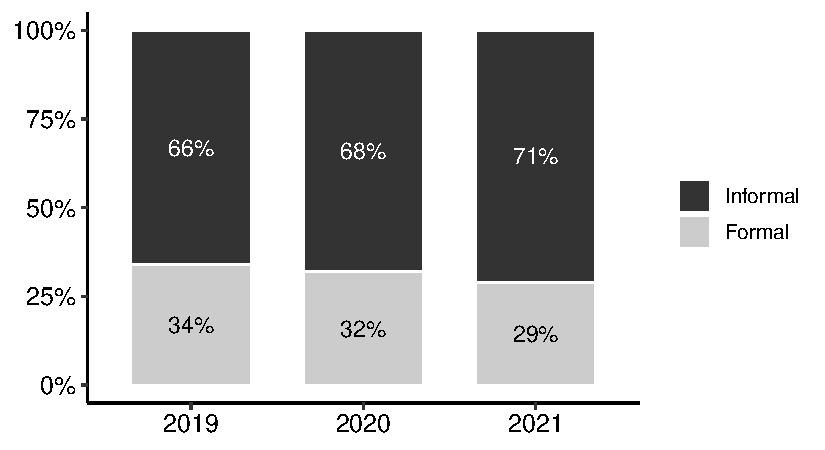
\includegraphics{Chapters/resultados_files/figure-pdf/fig-empleo-1.pdf}

}

\end{figure}

\noindent \small Fuente: Elaboración propia. \normalsize

El aumento del empleo informal ha sido experimentado con mayor
intensidad en la Selva Alta, la Sierra Centro y la Costa Sur, en los que
ha aumentado por lo menos en 7\% aprox. entre 2019 y 2021. En líneas
generales, el empleo informal aumentó en todos los dominios geográficos;
sin embargo, el aumento fue menor en Lima Metropolitana y en la Costa
Norte en los que se bordeó un aumento del 2\% en el empleo informal.

\hypertarget{tbl-dominio}{}
\begin{table}[H]
\caption{\label{tbl-dominio}Dominio de la PEA ocupada urbana entre 2019 y 2021 según informalidad
del empleo (porcentajes horizontales) }\tabularnewline

\centering\begingroup\fontsize{10}{12}\selectfont

\begin{tabular}{ccccccc}
\toprule
\multicolumn{1}{c}{ } & \multicolumn{2}{c}{\textbf{2019}} & \multicolumn{2}{c}{\textbf{2020}} & \multicolumn{2}{c}{\textbf{2021}} \\
\cmidrule(l{3pt}r{3pt}){2-3} \cmidrule(l{3pt}r{3pt}){4-5} \cmidrule(l{3pt}r{3pt}){6-7}
\textbf{Variable} & \textbf{Informal} & \textbf{Formal} & \textbf{Informal} & \textbf{Formal} & \textbf{Informal} & \textbf{Formal}\\
\midrule
\cellcolor{gray!6}{\textbf{Nacional}} & \cellcolor{gray!6}{66.40\%} & \cellcolor{gray!6}{33.60\%} & \cellcolor{gray!6}{68.42\%} & \cellcolor{gray!6}{31.58\%} & \cellcolor{gray!6}{71.41\%} & \cellcolor{gray!6}{28.59\%}\\
\textbf{Dominio Geográfico} &  &  &  &  &  & \\
\cellcolor{gray!6}{Costa Norte} & \cellcolor{gray!6}{72.53\%} & \cellcolor{gray!6}{27.47\%} & \cellcolor{gray!6}{72.42\%} & \cellcolor{gray!6}{27.58\%} & \cellcolor{gray!6}{74.56\%} & \cellcolor{gray!6}{25.44\%}\\
Costa Centro & 67.01\% & 32.99\% & 68.91\% & 31.09\% & 72.46\% & 27.54\%\\
\cellcolor{gray!6}{Costa Sur} & \cellcolor{gray!6}{68.12\%} & \cellcolor{gray!6}{31.88\%} & \cellcolor{gray!6}{67.92\%} & \cellcolor{gray!6}{32.08\%} & \cellcolor{gray!6}{73.02\%} & \cellcolor{gray!6}{26.98\%}\\
\addlinespace
Sierra Norte & 68.42\% & 31.58\% & 73.06\% & 26.94\% & 72.91\% & 27.09\%\\
\cellcolor{gray!6}{Sierra Centro} & \cellcolor{gray!6}{73.02\%} & \cellcolor{gray!6}{26.98\%} & \cellcolor{gray!6}{75.78\%} & \cellcolor{gray!6}{24.22\%} & \cellcolor{gray!6}{80.20\%} & \cellcolor{gray!6}{19.80\%}\\
Sierra Sur & 70.32\% & 29.68\% & 75.50\% & 24.50\% & 77.62\% & 22.38\%\\
\cellcolor{gray!6}{Selva Baja} & \cellcolor{gray!6}{74.84\%} & \cellcolor{gray!6}{25.16\%} & \cellcolor{gray!6}{80.69\%} & \cellcolor{gray!6}{19.31\%} & \cellcolor{gray!6}{83.04\%} & \cellcolor{gray!6}{16.96\%}\\
Selva Alta & 80.20\% & 19.80\% & 84.38\% & 15.62\% & 86.74\% & 13.26\%\\
\addlinespace
\cellcolor{gray!6}{Lima Metropolitana} & \cellcolor{gray!6}{58.60\%} & \cellcolor{gray!6}{41.40\%} & \cellcolor{gray!6}{58.22\%} & \cellcolor{gray!6}{41.78\%} & \cellcolor{gray!6}{61.99\%} & \cellcolor{gray!6}{38.01\%}\\
\bottomrule
\end{tabular}
\endgroup{}
\end{table}

\noindent \small Fuente: Elaboración propia. \normalsize

Asimismo, las ciudades de tamaño intermedio de entre 50 mil a 500 mil
habitantes no solo fueron parte de las que más perdieron trabajadores en
2020, sino que también se observa en la Tabla~\ref{tbl-estr} que
presentan un aumento en el empleo informal de 6\% aprox. entre 2019 y
2021. En segundo lugar, se encuentran las pequeñas ciudades de 2 mil a
20 mil habitantes que experimentaron un aumento de la informalidad en 5
puntos porcentuales.

\hypertarget{tbl-estr}{}
\begin{table}[H]
\caption{\label{tbl-estr}Estrato geográfico de la PEA ocupada urbana entre 2019 y 2021 según
informalidad del empleo (porcentajes horizontales) }\tabularnewline

\centering\begingroup\fontsize{10}{12}\selectfont

\begin{tabular}{ccccccc}
\toprule
\multicolumn{1}{c}{ } & \multicolumn{2}{c}{\textbf{2019}} & \multicolumn{2}{c}{\textbf{2020}} & \multicolumn{2}{c}{\textbf{2021}} \\
\cmidrule(l{3pt}r{3pt}){2-3} \cmidrule(l{3pt}r{3pt}){4-5} \cmidrule(l{3pt}r{3pt}){6-7}
\textbf{Variable} & \textbf{Informal} & \textbf{Formal} & \textbf{Informal} & \textbf{Formal} & \textbf{Informal} & \textbf{Formal}\\
\midrule
\cellcolor{gray!6}{\textbf{Nacional}} & \cellcolor{gray!6}{66.40\%} & \cellcolor{gray!6}{33.60\%} & \cellcolor{gray!6}{68.42\%} & \cellcolor{gray!6}{31.58\%} & \cellcolor{gray!6}{71.41\%} & \cellcolor{gray!6}{28.59\%}\\
\textbf{Habitantes} &  &  &  &  &  & \\
\cellcolor{gray!6}{500 000 a más} & \cellcolor{gray!6}{59.33\%} & \cellcolor{gray!6}{40.67\%} & \cellcolor{gray!6}{58.66\%} & \cellcolor{gray!6}{41.34\%} & \cellcolor{gray!6}{62.96\%} & \cellcolor{gray!6}{37.04\%}\\
100 000 - 499 999 & 68.31\% & 31.69\% & 71.41\% & 28.59\% & 74.75\% & 25.25\%\\
\cellcolor{gray!6}{50 000 - 99 999} & \cellcolor{gray!6}{69.71\%} & \cellcolor{gray!6}{30.29\%} & \cellcolor{gray!6}{73.73\%} & \cellcolor{gray!6}{26.27\%} & \cellcolor{gray!6}{75.64\%} & \cellcolor{gray!6}{24.36\%}\\
\addlinespace
20 000 - 49 999 & 74.31\% & 25.69\% & 76.15\% & 23.85\% & 76.55\% & 23.45\%\\
\cellcolor{gray!6}{2 000 - 19 999} & \cellcolor{gray!6}{78.12\%} & \cellcolor{gray!6}{21.88\%} & \cellcolor{gray!6}{81.60\%} & \cellcolor{gray!6}{18.40\%} & \cellcolor{gray!6}{83.40\%} & \cellcolor{gray!6}{16.60\%}\\
\bottomrule
\end{tabular}
\endgroup{}
\end{table}

\noindent \small Fuente: Elaboración propia. \normalsize

Con la finalidad de identificar de qué manera la pandemia afectó los
hogares conducidos por mujeres, la Tabla~\ref{tbl-sex} muestra la
distribución de la informalidad considerando el sexo del jefe de hogar.
Es así como se muestra que hay una predominancia de los hogares
conducidos por mujeres que se encuentran en el empleo informal. Si bien
han aumentado en el empleo informal tanto hogares conducidos por hombres
como aquellos conducidos por mujeres, se evidencia un mayor aumento en
el caso de los hombres con alrededor de 5\%.

\hypertarget{tbl-sex}{}
\begin{table}[H]
\caption{\label{tbl-sex}Sexo del jefe de hogar en la PEA ocupada urbana entre 2019 y 2021 según
informalidad del empleo (porcentajes horizontales) }\tabularnewline

\centering\begingroup\fontsize{10}{12}\selectfont

\begin{tabular}{ccccccc}
\toprule
\multicolumn{1}{c}{ } & \multicolumn{2}{c}{\textbf{2019}} & \multicolumn{2}{c}{\textbf{2020}} & \multicolumn{2}{c}{\textbf{2021}} \\
\cmidrule(l{3pt}r{3pt}){2-3} \cmidrule(l{3pt}r{3pt}){4-5} \cmidrule(l{3pt}r{3pt}){6-7}
\textbf{Variable} & \textbf{Informal} & \textbf{Formal} & \textbf{Informal} & \textbf{Formal} & \textbf{Informal} & \textbf{Formal}\\
\midrule
\cellcolor{gray!6}{\textbf{Nacional}} & \cellcolor{gray!6}{62.98\%} & \cellcolor{gray!6}{37.02\%} & \cellcolor{gray!6}{66.17\%} & \cellcolor{gray!6}{33.83\%} & \cellcolor{gray!6}{68.45\%} & \cellcolor{gray!6}{31.55\%}\\
\textbf{Sexo} &  &  &  &  &  & \\
\cellcolor{gray!6}{Hombre} & \cellcolor{gray!6}{60.09\%} & \cellcolor{gray!6}{39.91\%} & \cellcolor{gray!6}{63.52\%} & \cellcolor{gray!6}{36.48\%} & \cellcolor{gray!6}{65.98\%} & \cellcolor{gray!6}{34.02\%}\\
Mujer & 70.73\% & 29.27\% & 73.07\% & 26.93\% & 73.92\% & 26.08\%\\
\bottomrule
\end{tabular}
\endgroup{}
\end{table}

\noindent \small Fuente: Elaboración propia. \normalsize

En adición, los jefes de hogar entre 60 y 64 años tuvieron un aumento en
la informalidad de 7\% aproximadamente entre 2019 y 2021. En segundo
lugar, se encuentran los trabajadores entre 25 y 44 años quienes
aumentaron en alrededor de 6\%. Más aún, en el caso de este grupo, su
aumento fue más pronunciado dado que en 2020 presentó un aumento de
4.53\% en el empleo informal.

\hypertarget{tbl-gedad}{}
\begin{table}[H]
\caption{\label{tbl-gedad}Grupo de edad del jefe de hogar en la PEA ocupada urbana entre 2019 y
2021 según informalidad del empleo (porcentajes horizontales) }\tabularnewline

\centering\begingroup\fontsize{10}{12}\selectfont

\begin{tabular}{ccccccc}
\toprule
\multicolumn{1}{c}{ } & \multicolumn{2}{c}{\textbf{2019}} & \multicolumn{2}{c}{\textbf{2020}} & \multicolumn{2}{c}{\textbf{2021}} \\
\cmidrule(l{3pt}r{3pt}){2-3} \cmidrule(l{3pt}r{3pt}){4-5} \cmidrule(l{3pt}r{3pt}){6-7}
\textbf{Variable} & \textbf{Informal} & \textbf{Formal} & \textbf{Informal} & \textbf{Formal} & \textbf{Informal} & \textbf{Formal}\\
\midrule
\cellcolor{gray!6}{\textbf{Nacional}} & \cellcolor{gray!6}{62.98\%} & \cellcolor{gray!6}{37.02\%} & \cellcolor{gray!6}{66.17\%} & \cellcolor{gray!6}{33.83\%} & \cellcolor{gray!6}{68.45\%} & \cellcolor{gray!6}{31.55\%}\\
\textbf{Grupos de edad} &  &  &  &  &  & \\
\cellcolor{gray!6}{14-24} & \cellcolor{gray!6}{80.93\%} & \cellcolor{gray!6}{19.07\%} & \cellcolor{gray!6}{81.86\%} & \cellcolor{gray!6}{18.14\%} & \cellcolor{gray!6}{84.05\%} & \cellcolor{gray!6}{15.95\%}\\
25-44 & 62.73\% & 37.27\% & 67.26\% & 32.74\% & 68.34\% & 31.66\%\\
\cellcolor{gray!6}{45-59} & \cellcolor{gray!6}{58.30\%} & \cellcolor{gray!6}{41.70\%} & \cellcolor{gray!6}{61.78\%} & \cellcolor{gray!6}{38.22\%} & \cellcolor{gray!6}{64.65\%} & \cellcolor{gray!6}{35.35\%}\\
\addlinespace
60-64 & 61.77\% & 38.23\% & 63.64\% & 36.36\% & 68.86\% & 31.14\%\\
\cellcolor{gray!6}{65 a más} & \cellcolor{gray!6}{78.89\%} & \cellcolor{gray!6}{21.11\%} & \cellcolor{gray!6}{78.30\%} & \cellcolor{gray!6}{21.70\%} & \cellcolor{gray!6}{80.09\%} & \cellcolor{gray!6}{19.91\%}\\
\bottomrule
\end{tabular}
\endgroup{}
\end{table}

\noindent \small Fuente: Elaboración propia. \normalsize

En la Tabla~\ref{tbl-edpobre} se observó que respecto al nivel
educativo, los trabajadores con educación formal superior (técnico o
universitaria) tuvieron una lenta recuperación que no retomó los niveles
prepandemia. Asimismo, se constata en la Tabla~\ref{tbl-edu} que, dentro
de los jefes de hogar, los trabajadores con educación universitaria
incompleta en 2019 se encontraban casi en partes iguales tanto en la
formalidad como en la informalidad. Esa situación varió hacia 2021, en
la que 6 de cada 10 jefes de hogar con educación universitaria completa
cuentan con un empleo informal. De esta manera, se puede concluir que la
pandemia afectó sobre todo a aquellos que se encontraban en el proceso
de acentuarse dentro de una profesión.

\hypertarget{tbl-edu}{}
\begin{table}[H]
\caption{\label{tbl-edu}Nivel educativo alcanzado del jefe de hogar en la PEA ocupada urbana
entre 2019 y 2021 según informalidad del empleo (porcentajes
horizontales) }\tabularnewline

\centering\begingroup\fontsize{10}{12}\selectfont

\begin{tabular}{ccccccc}
\toprule
\multicolumn{1}{c}{ } & \multicolumn{2}{c}{\textbf{2019}} & \multicolumn{2}{c}{\textbf{2020}} & \multicolumn{2}{c}{\textbf{2021}} \\
\cmidrule(l{3pt}r{3pt}){2-3} \cmidrule(l{3pt}r{3pt}){4-5} \cmidrule(l{3pt}r{3pt}){6-7}
\textbf{Variable} & \textbf{Informal} & \textbf{Formal} & \textbf{Informal} & \textbf{Formal} & \textbf{Informal} & \textbf{Formal}\\
\midrule
\cellcolor{gray!6}{\textbf{Nacional}} & \cellcolor{gray!6}{62.98\%} & \cellcolor{gray!6}{37.02\%} & \cellcolor{gray!6}{66.17\%} & \cellcolor{gray!6}{33.83\%} & \cellcolor{gray!6}{68.45\%} & \cellcolor{gray!6}{31.55\%}\\
\textbf{Educación} &  &  &  &  &  & \\
\cellcolor{gray!6}{Sin nivel} & \cellcolor{gray!6}{92.71\%} & \cellcolor{gray!6}{7.29\%} & \cellcolor{gray!6}{93.52\%} & \cellcolor{gray!6}{6.48\%} & \cellcolor{gray!6}{95.58\%} & \cellcolor{gray!6}{4.42\%}\\
Secundaria incompleta o menos & 86.14\% & 13.86\% & 86.91\% & 13.09\% & 88.68\% & 11.32\%\\
\cellcolor{gray!6}{Secundaria completa} & \cellcolor{gray!6}{66.49\%} & \cellcolor{gray!6}{33.51\%} & \cellcolor{gray!6}{71.54\%} & \cellcolor{gray!6}{28.46\%} & \cellcolor{gray!6}{72.47\%} & \cellcolor{gray!6}{27.53\%}\\
\addlinespace
Técnica incompleta & 57.83\% & 42.17\% & 61.60\% & 38.40\% & 62.50\% & 37.50\%\\
\cellcolor{gray!6}{Técnica completa} & \cellcolor{gray!6}{39.25\%} & \cellcolor{gray!6}{60.75\%} & \cellcolor{gray!6}{38.92\%} & \cellcolor{gray!6}{61.08\%} & \cellcolor{gray!6}{42.80\%} & \cellcolor{gray!6}{57.20\%}\\
Universitaria incompleta & 51.07\% & 48.93\% & 58.63\% & 41.37\% & 58.55\% & 41.45\%\\
\cellcolor{gray!6}{Universitaria completa} & \cellcolor{gray!6}{25.03\%} & \cellcolor{gray!6}{74.97\%} & \cellcolor{gray!6}{24.89\%} & \cellcolor{gray!6}{75.11\%} & \cellcolor{gray!6}{26.88\%} & \cellcolor{gray!6}{73.12\%}\\
Posgrado & 9.06\% & 90.94\% & 8.12\% & 91.88\% & 8.14\% & 91.86\%\\
\bottomrule
\end{tabular}
\endgroup{}
\end{table}

\noindent \small Fuente: Elaboración propia. \normalsize

Alrededor del 80\% de quechuahablantes (y otras lenguas nativas) contaba
con un empleo informal. Esta situación no ha cambiado mucho dado que
hacia 2021 esta cifra aumentó en 2\%. En cambio, en el caso de los
trabajadores hispanohablantes, la llegada de la pandemia ocasionó un
aumento de hasta 5\% hacia el 2021.

\hypertarget{tbl-leng}{}
\begin{table}[H]
\caption{\label{tbl-leng}Lengua materna de la PEA ocupada urbana entre 2019 y 2021 según
informalidad del empleo (porcentajes horizontales) }\tabularnewline

\centering\begingroup\fontsize{10}{12}\selectfont

\begin{tabular}{ccccccc}
\toprule
\multicolumn{1}{c}{ } & \multicolumn{2}{c}{\textbf{2019}} & \multicolumn{2}{c}{\textbf{2020}} & \multicolumn{2}{c}{\textbf{2021}} \\
\cmidrule(l{3pt}r{3pt}){2-3} \cmidrule(l{3pt}r{3pt}){4-5} \cmidrule(l{3pt}r{3pt}){6-7}
\textbf{Variable} & \textbf{Informal} & \textbf{Formal} & \textbf{Informal} & \textbf{Formal} & \textbf{Informal} & \textbf{Formal}\\
\midrule
\cellcolor{gray!6}{\textbf{Nacional}} & \cellcolor{gray!6}{66.40\%} & \cellcolor{gray!6}{33.60\%} & \cellcolor{gray!6}{68.42\%} & \cellcolor{gray!6}{31.58\%} & \cellcolor{gray!6}{71.41\%} & \cellcolor{gray!6}{28.59\%}\\
\textbf{Lengua materna} &  &  &  &  &  & \\
\cellcolor{gray!6}{Castellano} & \cellcolor{gray!6}{64.60\%} & \cellcolor{gray!6}{35.40\%} & \cellcolor{gray!6}{66.01\%} & \cellcolor{gray!6}{33.99\%} & \cellcolor{gray!6}{69.80\%} & \cellcolor{gray!6}{30.20\%}\\
Quechua y otras lenguas nativas & 80.10\% & 19.90\% & 81.74\% & 18.26\% & 82.45\% & 17.55\%\\
\cellcolor{gray!6}{Otros} & \cellcolor{gray!6}{60.12\%} & \cellcolor{gray!6}{39.88\%} & \cellcolor{gray!6}{82.54\%} & \cellcolor{gray!6}{17.46\%} & \cellcolor{gray!6}{70.81\%} & \cellcolor{gray!6}{29.19\%}\\
\bottomrule
\end{tabular}
\endgroup{}
\end{table}

\noindent \small Fuente: Elaboración propia. \normalsize

El empleo informal presenta amplias diferencias dependiendo de la
categoría de ocupación principal del trabajador. Como se observa en la
Tabla~\ref{tbl-ocupi}, para el caso de los empleadores y obreros el
aumento en la informalidad ha sido mayor siendo alrededor de 5\%. En el
caso de los trabajadores independientes, se puede apreciar que el
aumento en la informalidad se estabiliza entre 2020 y 2021. Cabe
recalcar que los trabajadores familiares no remunerados están presentes
únicamente en el empleo informal, por definición.

\hypertarget{tbl-ocupi}{}
\begin{table}[H]
\caption{\label{tbl-ocupi}Ocupación principal de la PEA ocupada urbana entre 2019 y 2021 según
informalidad del empleo (porcentajes horizontales) }\tabularnewline

\centering\begingroup\fontsize{10}{12}\selectfont

\begin{tabular}{ccccccc}
\toprule
\multicolumn{1}{c}{ } & \multicolumn{2}{c}{\textbf{2019}} & \multicolumn{2}{c}{\textbf{2020}} & \multicolumn{2}{c}{\textbf{2021}} \\
\cmidrule(l{3pt}r{3pt}){2-3} \cmidrule(l{3pt}r{3pt}){4-5} \cmidrule(l{3pt}r{3pt}){6-7}
\textbf{Variable} & \textbf{Informal} & \textbf{Formal} & \textbf{Informal} & \textbf{Formal} & \textbf{Informal} & \textbf{Formal}\\
\midrule
\cellcolor{gray!6}{\textbf{Nacional}} & \cellcolor{gray!6}{66.40\%} & \cellcolor{gray!6}{33.60\%} & \cellcolor{gray!6}{68.42\%} & \cellcolor{gray!6}{31.58\%} & \cellcolor{gray!6}{71.41\%} & \cellcolor{gray!6}{28.59\%}\\
\textbf{Ocupación principal} &  &  &  &  &  & \\
\cellcolor{gray!6}{Empleador} & \cellcolor{gray!6}{45.73\%} & \cellcolor{gray!6}{54.27\%} & \cellcolor{gray!6}{47.22\%} & \cellcolor{gray!6}{52.78\%} & \cellcolor{gray!6}{50.81\%} & \cellcolor{gray!6}{49.19\%}\\
Independiente & 85.44\% & 14.56\% & 87.42\% & 12.58\% & 87.96\% & 12.04\%\\
\cellcolor{gray!6}{Empleado} & \cellcolor{gray!6}{36.68\%} & \cellcolor{gray!6}{63.32\%} & \cellcolor{gray!6}{34.02\%} & \cellcolor{gray!6}{65.98\%} & \cellcolor{gray!6}{39.84\%} & \cellcolor{gray!6}{60.16\%}\\
\addlinespace
Obrero & 69.88\% & 30.12\% & 70.34\% & 29.66\% & 74.12\% & 25.88\%\\
\cellcolor{gray!6}{Familiar No Remunerado} & \cellcolor{gray!6}{100.00\%} & \cellcolor{gray!6}{0.00\%} & \cellcolor{gray!6}{100.00\%} & \cellcolor{gray!6}{0.00\%} & \cellcolor{gray!6}{100.00\%} & \cellcolor{gray!6}{0.00\%}\\
Trabajador del Hogar & 88.03\% & 11.97\% & 86.29\% & 13.71\% & 91.87\% & 8.13\%\\
\cellcolor{gray!6}{Otro} & \cellcolor{gray!6}{100.00\%} & \cellcolor{gray!6}{0.00\%} & \cellcolor{gray!6}{100.00\%} & \cellcolor{gray!6}{0.00\%} & \cellcolor{gray!6}{100.00\%} & \cellcolor{gray!6}{0.00\%}\\
\bottomrule
\end{tabular}
\endgroup{}
\end{table}

\noindent \small Fuente: Elaboración propia. \normalsize

Respecto a la condición de pobreza, se observa que son los trabajadores
``no pobres'' quienes principalmente aumentaron su presencia en la
informalidad entre 2019 y 2021 en un 6\% aproximadamente. En el caso de
los pobres no extremos y extremos inclusive hubo una ligera disminución
de alrededor de 3\%, lo que puede denotar una expulsión del mercado
laboral.

\hypertarget{tbl-pobr}{}
\begin{table}[H]
\caption{\label{tbl-pobr}Condición de pobreza de la PEA ocupada urbana entre 2019 y 2021 según
informalidad del empleo (porcentajes horizontales) }\tabularnewline

\centering\begingroup\fontsize{10}{12}\selectfont

\begin{tabular}{ccccccc}
\toprule
\multicolumn{1}{c}{ } & \multicolumn{2}{c}{\textbf{2019}} & \multicolumn{2}{c}{\textbf{2020}} & \multicolumn{2}{c}{\textbf{2021}} \\
\cmidrule(l{3pt}r{3pt}){2-3} \cmidrule(l{3pt}r{3pt}){4-5} \cmidrule(l{3pt}r{3pt}){6-7}
\textbf{Variable} & \textbf{Informal} & \textbf{Formal} & \textbf{Informal} & \textbf{Formal} & \textbf{Informal} & \textbf{Formal}\\
\midrule
\cellcolor{gray!6}{\textbf{Nacional}} & \cellcolor{gray!6}{66.40\%} & \cellcolor{gray!6}{33.60\%} & \cellcolor{gray!6}{68.42\%} & \cellcolor{gray!6}{31.58\%} & \cellcolor{gray!6}{71.41\%} & \cellcolor{gray!6}{28.59\%}\\
\textbf{Pobreza} &  &  &  &  &  & \\
\cellcolor{gray!6}{Pobre Extremo} & \cellcolor{gray!6}{98.97\%} & \cellcolor{gray!6}{1.03\%} & \cellcolor{gray!6}{94.30\%} & \cellcolor{gray!6}{5.70\%} & \cellcolor{gray!6}{94.16\%} & \cellcolor{gray!6}{5.84\%}\\
Pobre No Extremo & 89.92\% & 10.08\% & 86.57\% & 13.43\% & 86.95\% & 13.05\%\\
\cellcolor{gray!6}{No Pobre} & \cellcolor{gray!6}{63.81\%} & \cellcolor{gray!6}{36.19\%} & \cellcolor{gray!6}{64.26\%} & \cellcolor{gray!6}{35.74\%} & \cellcolor{gray!6}{68.46\%} & \cellcolor{gray!6}{31.54\%}\\
\bottomrule
\end{tabular}
\endgroup{}
\end{table}

\noindent \small Fuente: Elaboración propia. \normalsize

\hypertarget{informalidad-y-condiciones-de-vida-ingreso-del-trabajador}{%
\section{Informalidad y condiciones de vida: ingreso del
trabajador}\label{informalidad-y-condiciones-de-vida-ingreso-del-trabajador}}

Según el INEI, para calcular el ingreso promedio por trabajador es
necesario separar a aquellos trabajadores que mensualmente generan cero
ingresos considerando su ocupación principal, secundaria, pago en
especias, entre otros. De esta manera, se puede realizar un cálculo
fidedigno equiparable al de los informes anuales presentados por esta
institución.

Durante la pandemia, se observa una caída en los ingresos, especialmente
en 2020, la cual no se ha recuperado del todo en 2021. Se observa una
mayor caída en el empleo informal con una disminución del 8\% hacia el
2020.

\break

\begin{figure}

\caption{\label{fig-pea_num}Ingreso promedio por trabajo mensual de la
PEA ocupada urbana entre 2019 y 2021 según informalidad del empleo}

{\centering 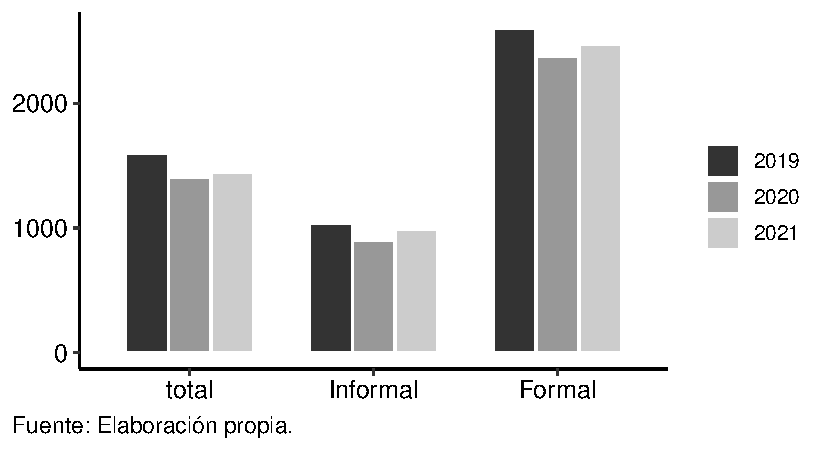
\includegraphics{Chapters/resultados_files/figure-pdf/fig-pea_num-1.pdf}

}

\end{figure}

\noindent \small Fuente: Elaboración propia. \normalsize

Asimismo, la variación en el ingreso tiene un impacto distinto
dependiendo de en qué región geográfica se encuentre el trabajador. La
Tabla~\ref{tbl-ing_dominio} muestra que, entre 2019 y 2021, los
trabajadores de Lima Metropolitana redujeron sus ingresos en s/.267
siendo los trabajadores con un empleo formal quienes fueron los más
perjudicados reduciendo su ingreso en s/.359. De igual manera, la Sierra
y la Costa Sur presentan una reducción importante de sus ingresos
alrededor de s/.200 mensuales. De esta manera, se muestra una reducción
del 14\% del ingreso promedio mensual con respecto al 2019.

Por otro lado, se observa cierta protección por parte de la formalidad
respecto al ingreso mensual en la Sierra Norte, la Selva y la Costa
centro. En estos casos, el ingreso promedio mensual aumentó, entre 2019
y 2021, en s/.504, s/. 288 y s/.171 respectivamente.

Cabe mencionar que se observa una irregularidad en el caso de la
categoría Selva Alta y Baja, en la que la diferencia del ingreso
promedio mensual a nivel general es negativa (1\%); y sin embargo, la
diferencia para el caso del empleo formal e informal en este sector es
positiva. Este posible error puede deberse a que es una categoría con
pocos casos, llevando a un error de muestreo, entre otras.

\hypertarget{tbl-ing_dominio}{}
\begin{table}[H]
\caption{\label{tbl-ing_dominio}Ingreso promedio por trabajo mensual (soles) de la PEA ocupada urbana
según dominio entre 2019 y 2021 según informalidad del empleo }\tabularnewline

\centering\begingroup\fontsize{9}{11}\selectfont

\begin{tabular}{cccccccccc}
\toprule
\multicolumn{1}{c}{ } & \multicolumn{3}{c}{\textbf{2019}} & \multicolumn{3}{c}{\textbf{2020}} & \multicolumn{3}{c}{\textbf{2021}} \\
\cmidrule(l{3pt}r{3pt}){2-4} \cmidrule(l{3pt}r{3pt}){5-7} \cmidrule(l{3pt}r{3pt}){8-10}
\textbf{Variable} & Total & \textbf{Informal} & \textbf{Formal} & Total & \textbf{Informal} & \textbf{Formal} & Total & \textbf{Informal} & \textbf{Formal}\\
\midrule
\cellcolor{gray!6}{\textbf{Nacional}} & \cellcolor{gray!6}{1,595} & \cellcolor{gray!6}{1,037} & \cellcolor{gray!6}{2,599} & \cellcolor{gray!6}{1,407} & \cellcolor{gray!6}{901} & \cellcolor{gray!6}{2,380} & \cellcolor{gray!6}{1,443} & \cellcolor{gray!6}{989} & \cellcolor{gray!6}{2,473}\\
\textbf{Dominio Geográfico} &  &  &  &  &  &  &  &  & \\
\cellcolor{gray!6}{Costa Norte} & \cellcolor{gray!6}{1,302} & \cellcolor{gray!6}{941} & \cellcolor{gray!6}{2,198} & \cellcolor{gray!6}{1,167} & \cellcolor{gray!6}{811} & \cellcolor{gray!6}{2,035} & \cellcolor{gray!6}{1,303} & \cellcolor{gray!6}{947} & \cellcolor{gray!6}{2,273}\\
Costa Centro & 1,398 & 1,033 & 2,072 & 1,317 & 962 & 2,051 & 1,376 & 1,022 & 2,243\\
\cellcolor{gray!6}{Costa Sur} & \cellcolor{gray!6}{1,560} & \cellcolor{gray!6}{1,071} & \cellcolor{gray!6}{2,518} & \cellcolor{gray!6}{1,390} & \cellcolor{gray!6}{918} & \cellcolor{gray!6}{2,317} & \cellcolor{gray!6}{1,401} & \cellcolor{gray!6}{1,008} & \cellcolor{gray!6}{2,397}\\
\addlinespace
Sierra Norte & 1,437 & 763 & 2,718 & 1,332 & 713 & 2,769 & 1,568 & 840 & 3,222\\
\cellcolor{gray!6}{Sierra Centro} & \cellcolor{gray!6}{1,339} & \cellcolor{gray!6}{845} & \cellcolor{gray!6}{2,454} & \cellcolor{gray!6}{1,276} & \cellcolor{gray!6}{706} & \cellcolor{gray!6}{2,694} & \cellcolor{gray!6}{1,209} & \cellcolor{gray!6}{804} & \cellcolor{gray!6}{2,588}\\
Sierra Sur & 1,475 & 977 & 2,505 & 1,256 & 835 & 2,290 & 1,273 & 879 & 2,433\\
\cellcolor{gray!6}{Selva Baja} & \cellcolor{gray!6}{1,343} & \cellcolor{gray!6}{909} & \cellcolor{gray!6}{2,476} & \cellcolor{gray!6}{1,205} & \cellcolor{gray!6}{870} & \cellcolor{gray!6}{2,400} & \cellcolor{gray!6}{1,327} & \cellcolor{gray!6}{999} & \cellcolor{gray!6}{2,731}\\
Selva Alta & 1,248 & 909 & 2,403 & 1,076 & 761 & 2,459 & 1,232 & 933 & 2,865\\
\addlinespace
\cellcolor{gray!6}{Lima Metropolitana} & \cellcolor{gray!6}{1,910} & \cellcolor{gray!6}{1,206} & \cellcolor{gray!6}{2,847} & \cellcolor{gray!6}{1,671} & \cellcolor{gray!6}{1,041} & \cellcolor{gray!6}{2,491} & \cellcolor{gray!6}{1,643} & \cellcolor{gray!6}{1,098} & \cellcolor{gray!6}{2,488}\\
\bottomrule
\end{tabular}
\endgroup{}
\end{table}

\noindent \small Fuente: Elaboración propia. \normalsize

De igual manera, se observa que principalmente las ciudades grandes,
aquellas con medio millón a más habitantes, han tenido una alta
disminución de sus ingresos de hasta s/.246. Esta caída ha sido más
pronunciada para el caso de los trabajadores formales que vieron sus
ingresos mensuales reducidos en s/.320. Resulta llamativo observar que
la protección de la formalidad es menor o nula para el caso de las
ciudades grandes, mientras que las pequeñas y medianas ciudades pudieron
mantener los empleos formales con un mayor ingreso, con un aumento del
6\% en los ingresos de las ciudades entre 20 mil a 50 mil habitantes
entre 2019 y 2021.

\hypertarget{tbl-ing_estrato}{}
\begin{table}[H]
\caption{\label{tbl-ing_estrato}Ingreso promedio por trabajo mensual (soles) de la PEA ocupada urbana
según estrato entre 2019 y 2021 según informalidad del empleo }\tabularnewline

\centering\begingroup\fontsize{9}{11}\selectfont

\begin{tabular}{cccccccccc}
\toprule
\multicolumn{1}{c}{ } & \multicolumn{3}{c}{\textbf{2019}} & \multicolumn{3}{c}{\textbf{2020}} & \multicolumn{3}{c}{\textbf{2021}} \\
\cmidrule(l{3pt}r{3pt}){2-4} \cmidrule(l{3pt}r{3pt}){5-7} \cmidrule(l{3pt}r{3pt}){8-10}
\textbf{Variable} & Total & \textbf{Informal} & \textbf{Formal} & Total & \textbf{Informal} & \textbf{Formal} & Total & \textbf{Informal} & \textbf{Formal}\\
\midrule
\cellcolor{gray!6}{\textbf{Nacional}} & \cellcolor{gray!6}{1,595} & \cellcolor{gray!6}{1,037} & \cellcolor{gray!6}{2,599} & \cellcolor{gray!6}{1,407} & \cellcolor{gray!6}{901} & \cellcolor{gray!6}{2,380} & \cellcolor{gray!6}{1,443} & \cellcolor{gray!6}{989} & \cellcolor{gray!6}{2,473}\\
\textbf{Habitantes} &  &  &  &  &  &  &  &  & \\
\cellcolor{gray!6}{500 000 a más} & \cellcolor{gray!6}{1,869} & \cellcolor{gray!6}{1,190} & \cellcolor{gray!6}{2,798} & \cellcolor{gray!6}{1,641} & \cellcolor{gray!6}{1,025} & \cellcolor{gray!6}{2,455} & \cellcolor{gray!6}{1,623} & \cellcolor{gray!6}{1,091} & \cellcolor{gray!6}{2,478}\\
100 000 - 499 999 & 1,438 & 959 & 2,375 & 1,310 & 887 & 2,259 & 1,382 & 954 & 2,538\\
\cellcolor{gray!6}{50 000 - 99 999} & \cellcolor{gray!6}{1,462} & \cellcolor{gray!6}{1,007} & \cellcolor{gray!6}{2,417} & \cellcolor{gray!6}{1,275} & \cellcolor{gray!6}{872} & \cellcolor{gray!6}{2,288} & \cellcolor{gray!6}{1,381} & \cellcolor{gray!6}{1,015} & \cellcolor{gray!6}{2,412}\\
\addlinespace
20 000 - 49 999 & 1,299 & 911 & 2,297 & 1,161 & 806 & 2,163 & 1,311 & 932 & 2,426\\
\cellcolor{gray!6}{2 000 - 19 999} & \cellcolor{gray!6}{1,192} & \cellcolor{gray!6}{853} & \cellcolor{gray!6}{2,234} & \cellcolor{gray!6}{1,098} & \cellcolor{gray!6}{742} & \cellcolor{gray!6}{2,364} & \cellcolor{gray!6}{1,148} & \cellcolor{gray!6}{846} & \cellcolor{gray!6}{2,420}\\
\bottomrule
\end{tabular}
\endgroup{}
\end{table}

\noindent \small Fuente: Elaboración propia. \normalsize

Respecto al ingreso mensual según educación, se confirma que los
trabajadores con un mayor grado de educación completo, ya sea técnica o
universitaria, presentan una menor variación en sus ingresos. En cambio,
los trabajadores con únicamente educación secundaria o estudios técnicos
incompletos vieron sus ingresos disminuidos en alrededor de s/.150 o 9\%
de su ingreso en comparación con el 2019. Esto guarda congruencia con el
estudio elaborado por Higa et~al.
(\protect\hyperlink{ref-higa2021}{2021}) en la que menciona un aumento
en la brecha de ingresos por hora entre los trabajadores con mayor
educación frente a los que tenían una menor a inicios de la pandemia.

Cabe destacar el caso atípico de los trabajadores con un grado de
posgrado que cuentan con un empleo informal. Si bien es una categoría
con pocos casos encuestados, entre 1000 y 1200 por año, sería
recomendable indagar más sobre el tipo de relaciones laborales que
establecen desde la informalidad: subcontratación, independientes sin
recibo por honorario, entre otros.

\hypertarget{tbl-ing_edu}{}
\begin{table}[H]
\caption{\label{tbl-ing_edu}Ingreso promedio por trabajo mensual (soles) de la PEA ocupada urbana
según educación entre 2019 y 2021 según informalidad del empleo }\tabularnewline

\centering\begingroup\fontsize{9}{11}\selectfont

\begin{tabular}{>{\centering\arraybackslash}p{10em}ccccccccc}
\toprule
\multicolumn{1}{c}{ } & \multicolumn{3}{c}{\textbf{2019}} & \multicolumn{3}{c}{\textbf{2020}} & \multicolumn{3}{c}{\textbf{2021}} \\
\cmidrule(l{3pt}r{3pt}){2-4} \cmidrule(l{3pt}r{3pt}){5-7} \cmidrule(l{3pt}r{3pt}){8-10}
\textbf{Variable} & Total & \textbf{Informal} & \textbf{Formal} & Total & \textbf{Informal} & \textbf{Formal} & Total & \textbf{Informal} & \textbf{Formal}\\
\midrule
\cellcolor{gray!6}{\textbf{Nacional}} & \cellcolor{gray!6}{1,595} & \cellcolor{gray!6}{1,037} & \cellcolor{gray!6}{2,599} & \cellcolor{gray!6}{1,407} & \cellcolor{gray!6}{901} & \cellcolor{gray!6}{2,380} & \cellcolor{gray!6}{1,443} & \cellcolor{gray!6}{989} & \cellcolor{gray!6}{2,473}\\
\textbf{Educación} &  &  &  &  &  &  &  &  & \\
\cellcolor{gray!6}{Sin nivel} & \cellcolor{gray!6}{597} & \cellcolor{gray!6}{520} & \cellcolor{gray!6}{1,610} & \cellcolor{gray!6}{586} & \cellcolor{gray!6}{533} & \cellcolor{gray!6}{1,544} & \cellcolor{gray!6}{569} & \cellcolor{gray!6}{527} & \cellcolor{gray!6}{1,709}\\
Secundaria incompleta o menos & 1,021 & 906 & 1,812 & 858 & 761 & 1,573 & 965 & 868 & 1,753\\
\cellcolor{gray!6}{Secundaria completa} & \cellcolor{gray!6}{1,367} & \cellcolor{gray!6}{1,085} & \cellcolor{gray!6}{2,068} & \cellcolor{gray!6}{1,164} & \cellcolor{gray!6}{921} & \cellcolor{gray!6}{1,833} & \cellcolor{gray!6}{1,224} & \cellcolor{gray!6}{1,011} & \cellcolor{gray!6}{1,902}\\
\addlinespace
Técnica incompleta & 1,356 & 998 & 2,061 & 1,282 & 873 & 2,086 & 1,245 & 951 & 1,876\\
\cellcolor{gray!6}{Técnica completa} & \cellcolor{gray!6}{1,789} & \cellcolor{gray!6}{1,162} & \cellcolor{gray!6}{2,291} & \cellcolor{gray!6}{1,635} & \cellcolor{gray!6}{983} & \cellcolor{gray!6}{2,131} & \cellcolor{gray!6}{1,681} & \cellcolor{gray!6}{1,075} & \cellcolor{gray!6}{2,254}\\
Universitaria incompleta & 1,487 & 969 & 2,228 & 1,349 & 948 & 2,043 & 1,370 & 997 & 2,054\\
\cellcolor{gray!6}{Universitaria completa} & \cellcolor{gray!6}{2,768} & \cellcolor{gray!6}{1,531} & \cellcolor{gray!6}{3,287} & \cellcolor{gray!6}{2,592} & \cellcolor{gray!6}{1,436} & \cellcolor{gray!6}{3,085} & \cellcolor{gray!6}{2,729} & \cellcolor{gray!6}{1,510} & \cellcolor{gray!6}{3,350}\\
Posgrado & 4,778 & 2,986 & 4,999 & 4,449 & 4,474 & 4,447 & 4,708 & 4,550 & 4,725\\
\bottomrule
\end{tabular}
\endgroup{}
\end{table}

\noindent \small Fuente: Elaboración propia. \normalsize

La Tabla~\ref{tbl-ing_sexo} nos permite apreciar que, si bien ha habido
una reducción del 10\% en el ingreso mensual tanto en hombres como en
mujeres trabajadoras, existen diferencias salariales cuando se considera
la participación de cada uno en la PEA ocupada urbana a través de un
empleo formal o informal. Por el lado de las mujeres, se observa que
tienen un ingreso menor al de los hombres que dista entre s/.300 y
s/.500 mensuales. Además, las mujeres con un empleo formal han
experimentado una mayor reducción de sus ingresos en un 7\% a diferencia
de sus pares con empleo informal. Por el lado de los hombres, se observa
que han tenido una mayor reducción de sus ingresos, en términos
generales, perdiendo hasta s/.180 en su ingreso mensual entre 2019 y
2021. Además, resulta llamativo que en el caso de los hombres aquellos
que tuvieron una mayor reducción de sus ingresos fueron los trabajadores
hombres informales con un 6\% menos entre 2019 y 2021.

\hypertarget{tbl-ing_sexo}{}
\begin{table}[H]
\caption{\label{tbl-ing_sexo}Ingreso promedio por trabajo mensual (soles) de la PEA ocupada urbana
según sexo entre 2019 y 2021 según informalidad del empleo }\tabularnewline

\centering\begingroup\fontsize{9}{11}\selectfont

\begin{tabular}{cccccccccc}
\toprule
\multicolumn{1}{c}{ } & \multicolumn{3}{c}{\textbf{2019}} & \multicolumn{3}{c}{\textbf{2020}} & \multicolumn{3}{c}{\textbf{2021}} \\
\cmidrule(l{3pt}r{3pt}){2-4} \cmidrule(l{3pt}r{3pt}){5-7} \cmidrule(l{3pt}r{3pt}){8-10}
\textbf{Variable} & Total & \textbf{Informal} & \textbf{Formal} & Total & \textbf{Informal} & \textbf{Formal} & Total & \textbf{Informal} & \textbf{Formal}\\
\midrule
\cellcolor{gray!6}{\textbf{Nacional}} & \cellcolor{gray!6}{1,595} & \cellcolor{gray!6}{1,037} & \cellcolor{gray!6}{2,599} & \cellcolor{gray!6}{1,407} & \cellcolor{gray!6}{901} & \cellcolor{gray!6}{2,380} & \cellcolor{gray!6}{1,443} & \cellcolor{gray!6}{989} & \cellcolor{gray!6}{2,473}\\
\textbf{Sexo} &  &  &  &  &  &  &  &  & \\
\cellcolor{gray!6}{Hombre} & \cellcolor{gray!6}{1,819} & \cellcolor{gray!6}{1,225} & \cellcolor{gray!6}{2,778} & \cellcolor{gray!6}{1,549} & \cellcolor{gray!6}{1,018} & \cellcolor{gray!6}{2,527} & \cellcolor{gray!6}{1,639} & \cellcolor{gray!6}{1,150} & \cellcolor{gray!6}{2,680}\\
Mujer & 1,308 & 816 & 2,327 & 1,203 & 739 & 2,154 & 1,183 & 784 & 2,168\\
\bottomrule
\end{tabular}
\endgroup{}
\end{table}

\noindent \small Fuente: Elaboración propia. \normalsize

\begin{figure}

\caption{\label{fig-ing_sexo}Diferencia del ingreso promedio por trabajo
mensual (soles) de la PEA ocupada urbana según sexo entre 2019 y 2021
según informalidad del empleo}

{\centering 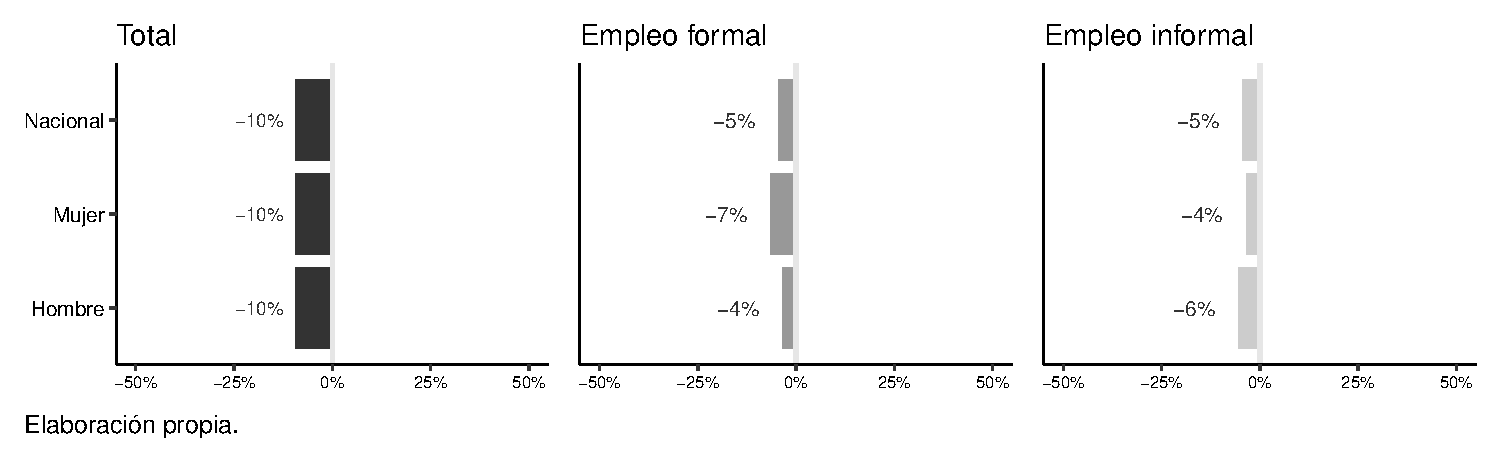
\includegraphics{Chapters/resultados_files/figure-pdf/fig-ing_sexo-1.pdf}

}

\end{figure}

\noindent \small Fuente: Elaboración propia. \normalsize

La Tabla~\ref{tbl-ing_gedad} nos muestra que, en líneas generales, los
trabajadores de 55 a 64 años vieron sus ingresos más comprometidos en
especial aquellos que contaban con un empleo formal. De similar manera,
los trabajadores entre 35 y 44 años vieron sus ingresos reducidos
principalmente los trabajadores formales. Cabe destacar, una ligera
recuperación de los ingresos en los trabajadores de 24 años a menos.

\break

\hypertarget{tbl-ing_gedad}{}
\begin{table}[H]
\caption{\label{tbl-ing_gedad}Ingreso promedio por trabajo mensual (soles) de la PEA ocupada urbana
según grupo de edad entre 2019 y 2021 según informalidad del empleo }\tabularnewline

\centering\begingroup\fontsize{9}{11}\selectfont

\begin{tabular}{cccccccccc}
\toprule
\multicolumn{1}{c}{ } & \multicolumn{3}{c}{\textbf{2019}} & \multicolumn{3}{c}{\textbf{2020}} & \multicolumn{3}{c}{\textbf{2021}} \\
\cmidrule(l{3pt}r{3pt}){2-4} \cmidrule(l{3pt}r{3pt}){5-7} \cmidrule(l{3pt}r{3pt}){8-10}
\textbf{Variable} & Total & \textbf{Informal} & \textbf{Formal} & Total & \textbf{Informal} & \textbf{Formal} & Total & \textbf{Informal} & \textbf{Formal}\\
\midrule
\cellcolor{gray!6}{\textbf{Nacional}} & \cellcolor{gray!6}{1,595} & \cellcolor{gray!6}{1,037} & \cellcolor{gray!6}{2,599} & \cellcolor{gray!6}{1,407} & \cellcolor{gray!6}{901} & \cellcolor{gray!6}{2,380} & \cellcolor{gray!6}{1,443} & \cellcolor{gray!6}{989} & \cellcolor{gray!6}{2,473}\\
\textbf{Grupos de edad} &  &  &  &  &  &  &  &  & \\
\cellcolor{gray!6}{14-24} & \cellcolor{gray!6}{960} & \cellcolor{gray!6}{819} & \cellcolor{gray!6}{1,516} & \cellcolor{gray!6}{924} & \cellcolor{gray!6}{763} & \cellcolor{gray!6}{1,551} & \cellcolor{gray!6}{965} & \cellcolor{gray!6}{848} & \cellcolor{gray!6}{1,583}\\
25-44 & 1,730 & 1,155 & 2,628 & 1,463 & 971 & 2,332 & 1,543 & 1,080 & 2,462\\
\cellcolor{gray!6}{45-59} & \cellcolor{gray!6}{1,793} & \cellcolor{gray!6}{1,085} & \cellcolor{gray!6}{2,837} & \cellcolor{gray!6}{1,599} & \cellcolor{gray!6}{950} & \cellcolor{gray!6}{2,617} & \cellcolor{gray!6}{1,595} & \cellcolor{gray!6}{1,024} & \cellcolor{gray!6}{2,669}\\
\addlinespace
60-64 & 1,644 & 935 & 2,838 & 1,386 & 761 & 2,427 & 1,413 & 844 & 2,601\\
\cellcolor{gray!6}{65 a más} & \cellcolor{gray!6}{1,015} & \cellcolor{gray!6}{693} & \cellcolor{gray!6}{2,183} & \cellcolor{gray!6}{1,088} & \cellcolor{gray!6}{605} & \cellcolor{gray!6}{2,763} & \cellcolor{gray!6}{1,010} & \cellcolor{gray!6}{618} & \cellcolor{gray!6}{2,590}\\
\bottomrule
\end{tabular}
\endgroup{}
\end{table}

\noindent \small Fuente: Elaboración propia. \normalsize

Los trabajadores de 60 a 64 años tuvieron una reducción en sus ingresos
del 14\% entre 2019 y 2021. Más aún, aquellos que se encontraban con un
empleo informal fueron los más afectados con una pérdida de s/.75 en su
ingreso mensual que, en relación con su ingreso en 2019, corresponde al
11\%. En cambio, los trabajadores formales de este grupo etario vieron
sus ingresos reducidos en s/.237 lo que corresponde al 8\% de su
anterior ingreso. En segundo lugar, se encuentran los trabajadores de 45
a 59 años con una reducción del 11\% de sus ingresos lo cual impactó en
mayor medida a los trabajadores formales con una reducción en s/.168.

Cabe destacar que los trabajadores de 14 a 24 años, los más jóvenes, si
bien su ingreso se sitúa por debajo de la remuneración mínima vital
(s/.1025), se muestra una ligera recuperación en los ingresos
equiparable al nivel prepandemia.

\hypertarget{tbl-ing_leng}{}
\begin{table}[H]
\caption{\label{tbl-ing_leng}Ingreso promedio por trabajo mensual (soles) de la PEA ocupada urbana
según lengua materna entre 2019 y 2021 según informalidad del empleo }\tabularnewline

\centering\begingroup\fontsize{9}{11}\selectfont

\begin{tabular}{>{\centering\arraybackslash}p{10em}ccccccccc}
\toprule
\multicolumn{1}{c}{ } & \multicolumn{3}{c}{\textbf{2019}} & \multicolumn{3}{c}{\textbf{2020}} & \multicolumn{3}{c}{\textbf{2021}} \\
\cmidrule(l{3pt}r{3pt}){2-4} \cmidrule(l{3pt}r{3pt}){5-7} \cmidrule(l{3pt}r{3pt}){8-10}
\textbf{Variable} & Total & \textbf{Informal} & \textbf{Formal} & Total & \textbf{Informal} & \textbf{Formal} & Total & \textbf{Informal} & \textbf{Formal}\\
\midrule
\cellcolor{gray!6}{\textbf{Nacional}} & \cellcolor{gray!6}{1,595} & \cellcolor{gray!6}{1,037} & \cellcolor{gray!6}{2,599} & \cellcolor{gray!6}{1,407} & \cellcolor{gray!6}{901} & \cellcolor{gray!6}{2,380} & \cellcolor{gray!6}{1,443} & \cellcolor{gray!6}{989} & \cellcolor{gray!6}{2,473}\\
\textbf{Lengua materna} &  &  &  &  &  &  &  &  & \\
\cellcolor{gray!6}{Castellano} & \cellcolor{gray!6}{1,645} & \cellcolor{gray!6}{1,050} & \cellcolor{gray!6}{2,627} & \cellcolor{gray!6}{1,453} & \cellcolor{gray!6}{911} & \cellcolor{gray!6}{2,398} & \cellcolor{gray!6}{1,493} & \cellcolor{gray!6}{1,011} & \cellcolor{gray!6}{2,496}\\
Quechua y otras lenguas nativas & 1,255 & 966 & 2,264 & 1,131 & 839 & 2,201 & 1,143 & 875 & 2,216\\
\cellcolor{gray!6}{Otros} & \cellcolor{gray!6}{2,050} & \cellcolor{gray!6}{1,410} & \cellcolor{gray!6}{2,918} & \cellcolor{gray!6}{1,610} & \cellcolor{gray!6}{1,399} & \cellcolor{gray!6}{2,416} & \cellcolor{gray!6}{1,657} & \cellcolor{gray!6}{970} & \cellcolor{gray!6}{3,062}\\
\bottomrule
\end{tabular}
\endgroup{}
\end{table}

\noindent \small Fuente: Elaboración propia. \normalsize

De igual manera, la reducción de los ingresos mensuales durante la
pandemia afectó principalmente a los trabajadores independientes
experimentando una disminución en 14\% entre 2019 y 2021. Más aún,
dentro de este sector los trabajadores formales tuvieron una mayor
reducción que sus pares con el informal teniendo una disminución de
s/.273. Seguido a ellos, los obreros formales vieron sus ingresos
reducidos en s/.165. Cabe mencionar que se filtraron a los trabajadores
familiares no remunerados y la categoría ``Otros'' dado que no contaban
con ingresos reportados.

\hypertarget{tbl-ing_p507}{}
\begin{table}[H]
\caption{\label{tbl-ing_p507}Ingreso promedio por trabajo mensual (soles) de la PEA ocupada urbana
según posición ocupacional entre 2019 y 2021 según informalidad del
empleo }\tabularnewline

\centering\begingroup\fontsize{9}{11}\selectfont

\begin{tabular}{cccccccccc}
\toprule
\multicolumn{1}{c}{ } & \multicolumn{3}{c}{\textbf{2019}} & \multicolumn{3}{c}{\textbf{2020}} & \multicolumn{3}{c}{\textbf{2021}} \\
\cmidrule(l{3pt}r{3pt}){2-4} \cmidrule(l{3pt}r{3pt}){5-7} \cmidrule(l{3pt}r{3pt}){8-10}
\textbf{Variable} & Total & \textbf{Informal} & \textbf{Formal} & Total & \textbf{Informal} & \textbf{Formal} & Total & \textbf{Informal} & \textbf{Formal}\\
\midrule
\cellcolor{gray!6}{\textbf{Nacional}} & \cellcolor{gray!6}{1,595} & \cellcolor{gray!6}{1,037} & \cellcolor{gray!6}{2,599} & \cellcolor{gray!6}{1,407} & \cellcolor{gray!6}{901} & \cellcolor{gray!6}{2,380} & \cellcolor{gray!6}{1,443} & \cellcolor{gray!6}{989} & \cellcolor{gray!6}{2,473}\\
\textbf{Ocupación principal} &  &  &  &  &  &  &  &  & \\
\cellcolor{gray!6}{Empleador} & \cellcolor{gray!6}{2,801} & \cellcolor{gray!6}{1,926} & \cellcolor{gray!6}{3,538} & \cellcolor{gray!6}{2,533} & \cellcolor{gray!6}{1,802} & \cellcolor{gray!6}{3,187} & \cellcolor{gray!6}{2,662} & \cellcolor{gray!6}{1,960} & \cellcolor{gray!6}{3,386}\\
Independiente & 1,003 & 868 & 1,797 & 813 & 709 & 1,531 & 858 & 767 & 1,524\\
\cellcolor{gray!6}{Empleado} & \cellcolor{gray!6}{2,288} & \cellcolor{gray!6}{1,229} & \cellcolor{gray!6}{2,900} & \cellcolor{gray!6}{2,260} & \cellcolor{gray!6}{1,240} & \cellcolor{gray!6}{2,784} & \cellcolor{gray!6}{2,252} & \cellcolor{gray!6}{1,288} & \cellcolor{gray!6}{2,886}\\
\addlinespace
Obrero & 1,397 & 1,116 & 2,050 & 1,217 & 992 & 1,747 & 1,307 & 1,104 & 1,885\\
\cellcolor{gray!6}{Trabajador del Hogar} & \cellcolor{gray!6}{1,063} & \cellcolor{gray!6}{982} & \cellcolor{gray!6}{1,657} & \cellcolor{gray!6}{985} & \cellcolor{gray!6}{908} & \cellcolor{gray!6}{1,476} & \cellcolor{gray!6}{1,057} & \cellcolor{gray!6}{1,006} & \cellcolor{gray!6}{1,633}\\
\bottomrule
\end{tabular}
\endgroup{}
\end{table}

\noindent \small Fuente: Elaboración propia. \normalsize

Al describir el ingreso de los trabajadores en situación de pobreza, se
puede apreciar que principalmente los trabajadores no pobres han visto
reducidos sus ingresos hasta en un 8\% con una pronunciada caída en
2020. Si bien se observa un aumento del sueldo medio dentro del sector
pobre extremo, esto sería un indicador de un descenso en la línea de
pobreza de los trabajadores considerados ``no pobre'' hacia la categoría
``pobre extremo'' de la cual no se ve mayor recuperación hacia 2020.

\hypertarget{tbl-ing_pobreza}{}
\begin{table}[H]
\caption{\label{tbl-ing_pobreza}Ingreso promedio por trabajo mensual (soles) de la PEA ocupada urbana
según situación de pobreza entre 2019 y 2021 según informalidad del
empleo }\tabularnewline

\centering\begingroup\fontsize{9}{11}\selectfont

\begin{tabular}{cccccccccc}
\toprule
\multicolumn{1}{c}{ } & \multicolumn{3}{c}{\textbf{2019}} & \multicolumn{3}{c}{\textbf{2020}} & \multicolumn{3}{c}{\textbf{2021}} \\
\cmidrule(l{3pt}r{3pt}){2-4} \cmidrule(l{3pt}r{3pt}){5-7} \cmidrule(l{3pt}r{3pt}){8-10}
\textbf{Variable} & Total & \textbf{Informal} & \textbf{Formal} & Total & \textbf{Informal} & \textbf{Formal} & Total & \textbf{Informal} & \textbf{Formal}\\
\midrule
\cellcolor{gray!6}{\textbf{Nacional}} & \cellcolor{gray!6}{1,595} & \cellcolor{gray!6}{1,037} & \cellcolor{gray!6}{2,599} & \cellcolor{gray!6}{1,407} & \cellcolor{gray!6}{901} & \cellcolor{gray!6}{2,380} & \cellcolor{gray!6}{1,443} & \cellcolor{gray!6}{989} & \cellcolor{gray!6}{2,473}\\
\textbf{Pobreza} &  &  &  &  &  &  &  &  & \\
\cellcolor{gray!6}{Pobre Extremo} & \cellcolor{gray!6}{555} & \cellcolor{gray!6}{551} & \cellcolor{gray!6}{815} & \cellcolor{gray!6}{550} & \cellcolor{gray!6}{526} & \cellcolor{gray!6}{864} & \cellcolor{gray!6}{682} & \cellcolor{gray!6}{646} & \cellcolor{gray!6}{1,168}\\
Pobre No Extremo & 889 & 795 & 1,603 & 830 & 718 & 1,446 & 917 & 809 & 1,537\\
\cellcolor{gray!6}{No Pobre} & \cellcolor{gray!6}{1,686} & \cellcolor{gray!6}{1,084} & \cellcolor{gray!6}{2,634} & \cellcolor{gray!6}{1,545} & \cellcolor{gray!6}{965} & \cellcolor{gray!6}{2,464} & \cellcolor{gray!6}{1,556} & \cellcolor{gray!6}{1,041} & \cellcolor{gray!6}{2,555}\\
\bottomrule
\end{tabular}
\endgroup{}
\end{table}

\noindent \small Fuente: Elaboración propia. \normalsize

\begin{figure}

\caption{\label{fig-ing_pobreza}Diferencia del ingreso promedio por
trabajo mensual (soles) de la PEA ocupada urbana según nivel de pobreza
entre 2019 y 2021 según informalidad del empleo}

{\centering 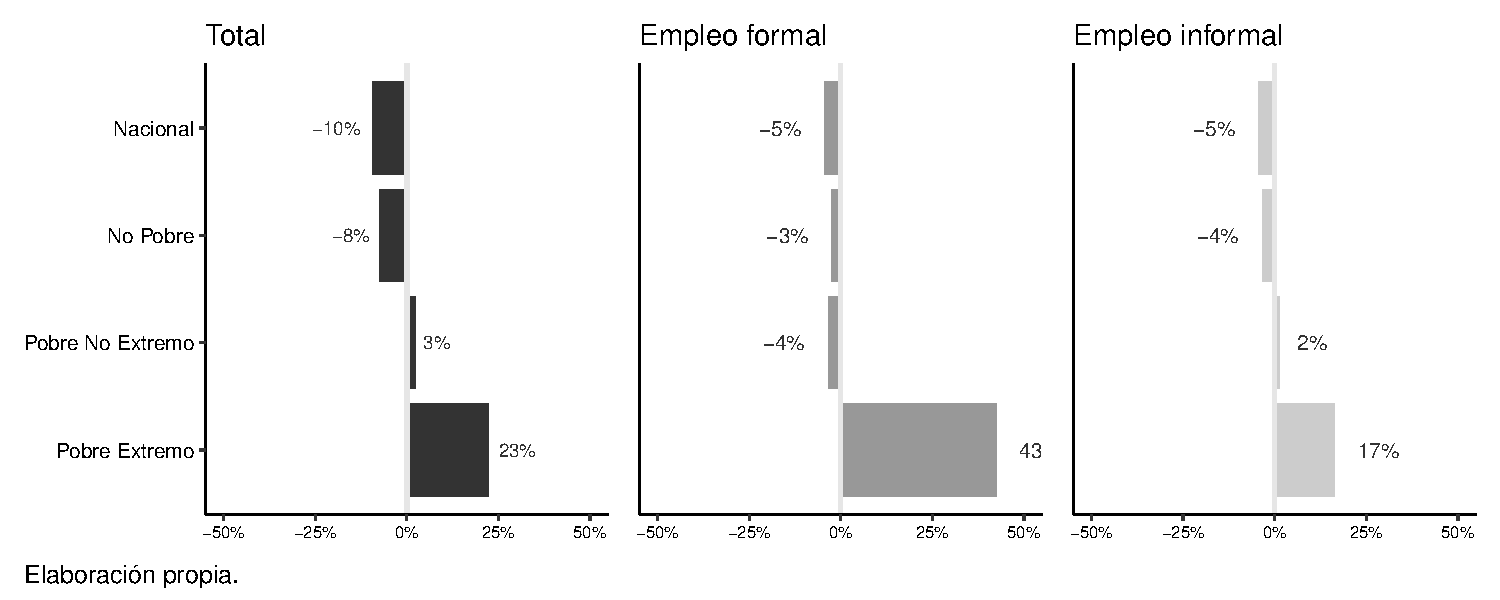
\includegraphics{Chapters/resultados_files/figure-pdf/fig-ing_pobreza-1.pdf}

}

\end{figure}

\noindent \small Fuente: Elaboración propia. \normalsize

\break

\bookmarksetup{startatroot}

\hypertarget{discusiuxf3n-y-conclusiones}{%
\chapter{Discusión y conclusiones}\label{discusiuxf3n-y-conclusiones}}

Los resultados presentados nos llevan a las siguientes conclusiones en
relación con las hipótesis planteadas:

En primer lugar, respecto a la hipótesis 1 - ``La pandemia ha aumentado
el empleo informal'': resultaría intuitivo responder que sí es el caso.
Efectivamente, se ha podido observar que el empleo informal ha aumentado
entre 2019 y 2021 en un 5\%; sin embargo, esta hipótesis se podría
aceptar de manera parcial; ya que, en términos absolutos, en el año 2020
(inicio de la pandemia) se perdieron alrededor de un millón doscientos
empleos informales y 900 mil empleos formales. Esta pérdida de empleo
fue más pronunciada en Lima Metropolitana y la Costa Norte. No obstante,
en 2021, hubo una recuperación del empleo informal que superó el nivel
prepandemia lo cual no fue el caso del empleo formal. Por lo que podemos
concluir que durante la pandemia tanto el empleo formal como informal se
vieron reducidos, mas el empleo informal pudo recuperarse hacia 2021.

En segundo lugar, la hipótesis 2 corresponde a la afirmación sobre si el
incremento del empleo informal se dio principalmente en zonas y grupos
vulnerables, especialmente: A) zonas urbanas de la Sierra y Selva, B)
ciudades de pequeña y mediana escala, C) entre jóvenes y mujeres, D)
entre los trabajadores con menor nivel educativo.

Considerando que nos referimos a un aumento del empleo informal en
términos relativos, hemos podido observar que:

\begin{enumerate}
\def\labelenumi{\Alph{enumi})}
\item
  Efectivamente ha aumentado la informalidad especialmente en la Selva
  Alta, Sierra Centro y la Costa Sur. En cambio, fue menor el aumento de
  empleo informal en lugares como Lima Metropolitana y la Costa Norte;
  sin embargo, en estas zonas destacó la pérdida de empleo en general.
\item
  Hacia el 2021, sobre todo las ciudades medianas de entre 50 mil y 500
  mil habitantes no solo tuvieron una amplia pérdida de empleo, sino que
  también se constata un aumento de la informalidad. En el caso de los
  trabajadores con empleo formal, estos vieron su sueldo reducido en
  mayor proporción que los trabajadores informales salvo en las ciudades
  pequeñas y medianas. En cambio, en la ciudades grandes la protección
  de los salarios formales fue mucho menor.
\item
  Se observó que 7 de cada 10 mujeres que eran jefas de hogar se
  encontraban en la informalidad, demostrando que hay una predominancia
  de hogares conducidos por mujeres que se encuentran en la
  informalidad. No obstante, se evidenció un mayor aumento de hombres
  jefes de hogar durante la pandemia con alrededor de 5\% entre 2019 y
  2021. Durante la pandemia, se observa que 1 de cada 7 hombres
  trabajadores perdieron su empleo, mientras que 1 de cada 5 mujeres
  perdieron su empleo. Si bien hacia 2021, se muestra una recuperación
  tanto en hombres como mujeres; no obstante, es más lenta en el caso de
  las trabajadoras. Asimismo, se pudo corroborar que en primera
  instancia fueron los jefes de hogar entre 60 y 64 años quienes fueron
  los más afectados, seguido de los adultos jóvenes entre 25 y 44 años
  lo que se alinea con la hipótesis de Higa et~al.
  (\protect\hyperlink{ref-higa2021}{2021}). Cabe mencionar que, en la
  pandemia se muestra un aumento de los trabajadores familiares no
  remunerados, lo cual podría ser un indicador de la recomposición en
  las labores del hogar optando por emplear trabajadores familiares sin
  paga alguna para sortear los impactos de la pandemia.
\item
  Los trabajadores que perdieron más puestos laborales fueron aquellos
  que contaban con una educación superior técnica o profesional y su
  recuperación fue lenta, de lo que podemos concluir que el título
  académico no necesariamente garantiza la continuidad de un puesto
  laboral. En cambio, sí se observa una cierta estabilidad en el ingreso
  mensual de los profesionales con estudios superiores que continuaron
  siendo empleados entre 2019 y 2021. Por otro lado, hacia 2021, aumentó
  el empleo informal principalmente en los trabajadores con educación
  universitaria incompleta o con educación secundaria, es decir, que la
  pandemia afectó sobre todo a aquellos que se encontraban en el proceso
  de acentuarse en una profesión.
\end{enumerate}

En tercer lugar, sobre la hipótesis 3 sobre si la pandemia ha tenido un
efecto negativo en el salario sobre todo del trabajador informal, vemos
que ciertamente ocurrió un deterioro importante del ingreso promedio
mensual reduciéndose en s/.152 entre 2019 y 2021. Ahora bien, esta
reducción representó el 5\% del ingreso promedio mensual tanto para los
trabajadores formales como informales, lo cual se refleja en s/.126 y
s/.48 menos respectivamente.

En cuarto lugar, la hipótesis 4 menciona que el deterioro del ingreso ha
sido mayor en los grupos más vulnerables como jóvenes y las personas de
menor nivel educativo. Sobre este punto, cabe mencionar que
principalmente los trabajadores formales de 60 a 64 años vieron sus
ingresos comprometidos. De manera similar, los trabajadores formales de
45 a 59 años redujeron sus ingresos. Por el contrario, cabe destacar una
ligera recuperación de los ingresos en los trabajadores de 24 años a
menos, pero que, sin embargo, permanecen ganando por debajo de la
remuneración mínima vital.

A modo de cierre, respecto a la pregunta: ¿cómo la pandemia del COVID-19
ha afectado las condiciones de vida de la Población Económicamente
Activa Ocupada (PEAO) urbana, específicamente los cambios en los
trabajadores con empleo informal?, podemos concluir que ciertamente la
pandemia ha conllevado un deterioro de las condiciones de vida
representadas en el ingreso. Sobre todo, se observó que si bien el
empleo informal recibió un duro choque durante la pandemia, hacia 2021
mostraba niveles de empleo similares a los prepandemia. Sin embargo,
principalmente tanto las mujeres jefas de hogar como los trabajadores
entre 60 y 64 años no han logrado reestablecer y/o superar la situación
previa a la pandemia.

\bookmarksetup{startatroot}

\hypertarget{bibliografuxeda}{%
\chapter*{Bibliografía}\label{bibliografuxeda}}
\addcontentsline{toc}{chapter}{Bibliografía}

\markboth{Bibliografía}{Bibliografía}

\hypertarget{refs}{}
\begin{CSLReferences}{1}{0}
\leavevmode\vadjust pre{\hypertarget{ref-acemoglu2001}{}}%
Acemoglu, D. (2001). Good jobs versus bad jobs. \emph{Chicago},
\emph{vol.19}(N°1).

\leavevmode\vadjust pre{\hypertarget{ref-alonso1990}{}}%
Alonso, J. A. (1990). Review of The Informal Economy. Studies in
Advanced and Less Developed Countries. \emph{Estudios Sociológicos},
\emph{8}(22), 191-197. \url{http://www.jstor.org/stable/40420059}

\leavevmode\vadjust pre{\hypertarget{ref-barco2010}{}}%
Barco, D., \& Vargas, P. (2010). \emph{DT 2010 04: El Perfil del
Trabajador Informal y el Retorno de la Educación}.
\url{https://www.bcrp.gob.pe/publicaciones/documentos-de-trabajo/dt-2010-04.html}

\leavevmode\vadjust pre{\hypertarget{ref-beiner1989}{}}%
Beiner, B. (1989). \emph{A Economia Invis{ı}vel {\textemdash} Um
Survey}.

\leavevmode\vadjust pre{\hypertarget{ref-belapatiuxf1o2017}{}}%
Belapatiño, V., Grippa, F., \& Perea, H. (2017). \emph{Perú \textbar{}
Informalidad laboral y algunas propuestas para reducirla}. 21.

\leavevmode\vadjust pre{\hypertarget{ref-beteta2020}{}}%
Beteta, H. E. (2020). ¿Cómo encontró la pandemia del Covid-19 a América
Latina? / How did you find the Covid-19 pandemic in Latin America?
\emph{EconomíaUNAM}, \emph{17}(51), 180-193.
\url{https://doi.org/10.22201/fe.24488143e.2020.51.556}

\leavevmode\vadjust pre{\hypertarget{ref-cacciamali1983}{}}%
Cacciamali, M. C. (1983). \emph{Setor Informal Urbano e Formas de
Participaçao}. \emph{N. 20}.

\leavevmode\vadjust pre{\hypertarget{ref-carneiro1997}{}}%
Carneiro, F. (1997). The Changing Informal Labour Market in Brazil:
Cyclicality versus Excessive Intervention. \emph{LABOUR}, \emph{11}(1),
3-22. \url{https://doi.org/10.1111/1467-9914.00027}

\leavevmode\vadjust pre{\hypertarget{ref-cartaya1987}{}}%
Cartaya, V. (1987). El Confuso Mundo del Sector Informal.
\emph{Jul/Ago}, \emph{N. 90}.

\leavevmode\vadjust pre{\hypertarget{ref-cuxe9spedesreynaga2020}{}}%
Céspedes Reynaga, N. (2020). \emph{Crecer no es suficiente para reducir
la informalidad}. Universidad de San Martín de Porres.
\url{https://repositorio.usmp.edu.pe/handle/20.500.12727/8844}

\leavevmode\vadjust pre{\hypertarget{ref-chacaltana2016}{}}%
Chacaltana, J. (2016). \emph{Perú, 2002-2012: crecimiento, cambio
estructural y formalización}. CEPAL.
\url{https://www.cepal.org/es/publicaciones/40402-peru-2002-2012-crecimiento-cambio-estructural-formalizacion}

\leavevmode\vadjust pre{\hypertarget{ref-cosamaluxf3n2018}{}}%
Cosamalón, J. (2018). \emph{El apocalipsis a la vuelta de la esquina}.
Fondo Editorial, PUCP.

\leavevmode\vadjust pre{\hypertarget{ref-durand2007}{}}%
Durand, F. (2007). \emph{3. Las tres economías}. Fondo Editorial del
Congreso del Perú.

\leavevmode\vadjust pre{\hypertarget{ref-elcomercio2021}{}}%
El Comercio. (2021). Recuperación de la producción e informalización del
empleo, por Miguel Jaramillo \textbar{} Opinión \textbar{} ECONOMIA.
\emph{El Comercio Perú}.
\url{https://elcomercio.pe/economia/peru/recuperacion-de-la-produccion-e-informalizacion-del-empleo-por-miguel-jaramillo-opinion-noticia/}

\leavevmode\vadjust pre{\hypertarget{ref-esquivel2011}{}}%
Esquivel, A. (2011). \emph{Cofopri ¿organismo diseñado para mejorar el
bienestar de las personas?}
\url{http://repositorio.flacsoandes.edu.ec/handle/10469/2842}

\leavevmode\vadjust pre{\hypertarget{ref-hart1971}{}}%
Hart, K. (1971). Informal Income Opportunities and Urban Employment in
Ghana. \emph{unpublished}.

\leavevmode\vadjust pre{\hypertarget{ref-higa2021}{}}%
Higa, M., Ospino, C., \& Aragon, F. (2021). \emph{The persistent effects
of COVID-19 on labor outcomes: evidence from Peru}.
\url{https://ideas.repec.org/p/sfu/sfudps/dp21-10.html}

\leavevmode\vadjust pre{\hypertarget{ref-inei2010}{}}%
INEI. (2010). \emph{Evolución de la Pobreza al 2010}.

\leavevmode\vadjust pre{\hypertarget{ref-inei2020}{}}%
INEI. (2020). \emph{PERÚ: Evolución de los Indicadores de Empleo e
Ingreso por Departamento, 2007-2019}.

\leavevmode\vadjust pre{\hypertarget{ref-inei2021}{}}%
INEI. (2021). \emph{Perú: Evolución de los Indicadores de Empleo e
Ingreso por departamento, 2007-2020}.

\leavevmode\vadjust pre{\hypertarget{ref-ipe2020}{}}%
IPE. (2020). \emph{Mercado laboral peruano: impacto por covid-19 y
recomendaciones de política}.

\leavevmode\vadjust pre{\hypertarget{ref-loayza2020}{}}%
Loayza, N. V. (2020). \emph{Informalidad y crecimiento económico: Una
aproximación conceptual y una aplicación al Perú}. Universidad de San
Martín de Porres.
\url{https://repositorio.usmp.edu.pe/handle/20.500.12727/8843}

\leavevmode\vadjust pre{\hypertarget{ref-mantilla2021}{}}%
Mantilla, E. (2021). \emph{¿Y qué será de la vida?: un análisis de las
diferentes dimensiones de la vulnerabilidad a la pobreza de los hogares
peruanos, 2014-19}.

\leavevmode\vadjust pre{\hypertarget{ref-oecd2004}{}}%
OECD. (2004). \emph{Informal Employment and Promoting the Transition to
a Salaried Economy} (pp. 225-289).
\url{https://doi.org/10.1787/empl_outlook-2004-7-en}

\leavevmode\vadjust pre{\hypertarget{ref-oit2002}{}}%
OIT. (2002). \emph{Report VI: Decent work and informal economy}.

\leavevmode\vadjust pre{\hypertarget{ref-oit2021}{}}%
OIT. (2021). \emph{Transition from the informal to the formal economy -
Theory of Change}.
\url{https://www.ilo.org/wcmsp5/groups/public/---ed_protect/---protrav/---travail/documents/briefingnote/wcms_768807.pdf}

\leavevmode\vadjust pre{\hypertarget{ref-puxe9rez-suxe1nchez1995}{}}%
Pérez-Sánchez, A. (1995). Deuda externa de América Latina. Balance de
una década (1980-1990). \emph{Cuadernos de Estudios Empresariales},
243-269.

\leavevmode\vadjust pre{\hypertarget{ref-piore1987}{}}%
Piore, M. J., \& Sabel, C. F. (1987). The Second Industrial Divide.
\emph{Journal of Peace Research}, \emph{24}(2), 354 pp.
\url{https://doi.org/10.1177/002234338702400213}

\leavevmode\vadjust pre{\hypertarget{ref-theinfo1989}{}}%
Portes, A., Castells, M., \& Benton, L. A. (Eds.). (1989). \emph{The
Informal economy: studies in advanced and less developed countries}.
Johns Hopkins University Press.

\leavevmode\vadjust pre{\hypertarget{ref-rodruxedguez2010}{}}%
Rodríguez, J., \& Higa, M. (2010). Informalidad, empleo y productividad
en el Perú. \emph{Departamento de Economía}, \emph{Documento de Trabajo
282}.

\leavevmode\vadjust pre{\hypertarget{ref-sanchuxe9zvillagomez2019}{}}%
Sanchéz Villagomez, M., \& Chafloque Céspedes, M. R. (2019). \emph{La
informalidad laboral en el Perú: un mapa nacional basado en ENAHO}.
Universidad San Martín de Porres.
\url{https://www.administracion.usmp.edu.pe/investigacion/files/INFORMALIDAD-LABORAL-final-corregido.pdf}

\leavevmode\vadjust pre{\hypertarget{ref-desoto1987}{}}%
Soto, H. de, Ghersi, E., \& Ghibellini, M. (1987). \emph{El otro
sendero}. \url{https://books.google.com.pe/books?id=ZU95PQAACAAJ}

\leavevmode\vadjust pre{\hypertarget{ref-soto2020}{}}%
Soto, R. M., Cuéllar, N. G., \& Reyes-Olivo, M. (2020). Empleo y derecho
laboral en tiempos de pandemia, Perú 2020. \emph{Ciencia Latina Revista
Científica Multidisciplinar}, \emph{4}(2), 1497-1509.
\url{https://doi.org/10.37811/cl_rcm.v4i2.156}

\leavevmode\vadjust pre{\hypertarget{ref-souza1980}{}}%
Souza, P. R. (1980). Emprego, Salários e Pobreza. \emph{Hucitec,
Brazil}.

\leavevmode\vadjust pre{\hypertarget{ref-tokman1978}{}}%
Tokman, V. (1978). \emph{Las Relaciones entre los Sectores Formal e
Informal: Una Exploraci´on sobre su Natureza}. \emph{N. 5}.

\leavevmode\vadjust pre{\hypertarget{ref-torres2019}{}}%
Torres, D., \& Ruiz-Tagle, J. (2019). ¿Derecho a la vivienda o la
propiedad privada? De la política pública a la informalidad urbana en el
Área Metropolitana de Lima (1996-2015). \emph{136}, 5-29.

\leavevmode\vadjust pre{\hypertarget{ref-toussaint2004}{}}%
Toussaint, E. (2004). \emph{Capítulo 7. La crisis de la deuda del Tercer
Mundo durante el período 1980-1990}. CLACSO, Consejo Latinoamericano de
Ciencias Sociales.

\leavevmode\vadjust pre{\hypertarget{ref-waldinger1985}{}}%
Waldinger, R., Ward, R., \& Aldrich, H. (1985). Ethnic Business and
Occupational Mobility in Advanced Societies. \emph{Sociology},
\emph{19}(4), 586-597. \url{https://doi.org/10.1177/0038038585019004007}

\end{CSLReferences}

\appendix
\addcontentsline{toc}{part}{Apéndices}

\hypertarget{sec-appA}{%
\chapter{Código anexado}\label{sec-appA}}

El código utilizado para realizar los gráficos y las tablas puede
encontrarse en el siguiente
\href{https://santiagosotelo.netlify.app/posts/03_tablas4_tesis/}{link}.



\end{document}
